\documentclass{beamer}\usepackage[]{graphicx}\usepackage[]{color}
%% maxwidth is the original width if it is less than linewidth
%% otherwise use linewidth (to make sure the graphics do not exceed the margin)
\makeatletter
\def\maxwidth{ %
  \ifdim\Gin@nat@width>\linewidth
    \linewidth
  \else
    \Gin@nat@width
  \fi
}
\makeatother

\definecolor{fgcolor}{rgb}{1, 0.894, 0.769}
\newcommand{\hlnum}[1]{\textcolor[rgb]{0.824,0.412,0.118}{#1}}%
\newcommand{\hlstr}[1]{\textcolor[rgb]{1,0.894,0.71}{#1}}%
\newcommand{\hlcom}[1]{\textcolor[rgb]{0.824,0.706,0.549}{#1}}%
\newcommand{\hlopt}[1]{\textcolor[rgb]{1,0.894,0.769}{#1}}%
\newcommand{\hlstd}[1]{\textcolor[rgb]{1,0.894,0.769}{#1}}%
\newcommand{\hlkwa}[1]{\textcolor[rgb]{0.941,0.902,0.549}{#1}}%
\newcommand{\hlkwb}[1]{\textcolor[rgb]{0.804,0.776,0.451}{#1}}%
\newcommand{\hlkwc}[1]{\textcolor[rgb]{0.78,0.941,0.545}{#1}}%
\newcommand{\hlkwd}[1]{\textcolor[rgb]{1,0.78,0.769}{#1}}%
\let\hlipl\hlkwb

\usepackage{framed}
\makeatletter
\newenvironment{kframe}{%
 \def\at@end@of@kframe{}%
 \ifinner\ifhmode%
  \def\at@end@of@kframe{\end{minipage}}%
  \begin{minipage}{\columnwidth}%
 \fi\fi%
 \def\FrameCommand##1{\hskip\@totalleftmargin \hskip-\fboxsep
 \colorbox{shadecolor}{##1}\hskip-\fboxsep
     % There is no \\@totalrightmargin, so:
     \hskip-\linewidth \hskip-\@totalleftmargin \hskip\columnwidth}%
 \MakeFramed {\advance\hsize-\width
   \@totalleftmargin\z@ \linewidth\hsize
   \@setminipage}}%
 {\par\unskip\endMakeFramed%
 \at@end@of@kframe}
\makeatother

\definecolor{shadecolor}{rgb}{.97, .97, .97}
\definecolor{messagecolor}{rgb}{0, 0, 0}
\definecolor{warningcolor}{rgb}{1, 0, 1}
\definecolor{errorcolor}{rgb}{1, 0, 0}
\newenvironment{knitrout}{}{} % an empty environment to be redefined in TeX

\usepackage{alltt}
\usepackage{../371g-slides}
\title{Diagnostics \& Transformations 2}
\subtitle{Lecture 13}
\author{STA 371G}
\IfFileExists{upquote.sty}{\usepackage{upquote}}{}
\begin{document}
  
  

  \frame{\maketitle}

  % Show outline at beginning of each section
  \AtBeginSection[]{ 
    \begin{frame}<beamer>
      \tableofcontents[currentsection]
    \end{frame}
  }

  %%%%%%% Slides start here %%%%%%%

  \begin{darkframes}
    
    
    \begin{frame}
      \fontsize{8}{8}\selectfont
      Newly hired manager salaries
      \begin{center}
        \includegraphics[width=2.8in]{manager} \\
      \end{center} \pause
      
      \begin{columns}[onlytextwidth]
        \column{.5\textwidth}
          \begin{itemize}
            \item Salary (response)
            \item Manager Rating
          \end{itemize}
        \column{.5\textwidth}
          \begin{itemize}
            \item Years of Experience
            \item Origin (internal or external hire)
          \end{itemize}
      \end{columns}
    \end{frame}
      
   
   
   
   \begin{frame}[fragile]{Data issues}
    \fontsize{8}{8}\selectfont
      \begin{center}
          It is extremely rare that the data could be used right away without any clean up. \bigskip \pause
          
          Data scients report that they spend \alert{70\% of their time on getting and cleaning the data}. Only 30\% is for statistical analysis.\bigskip \pause
          
          Most common issues are:
          
          
        
          \parbox{.43\textwidth}{
          \begin{itemize}[<+->]
            \item Outliers (e.g. incorrect entries, anomalies)
            \item Missing data
            \item Multicollinearity
            \item Violation of LINE assumptions
          \end{itemize}} \bigskip \pause
          
          It is almost always necessary to explore the data before doing the modeling
          
      \end{center}
      
    \end{frame}
    
    
    
    
    \begin{frame}[fragile]%{Exploring the data: Outliers}
      \fontsize{8}{8}\selectfont
      Boxplots are commonly used to detect the outliers. \pause
      
      Let's start with looking into the salary column. \pause
      
\begin{knitrout}
\definecolor{shadecolor}{rgb}{0.137, 0.137, 0.137}\begin{kframe}
\begin{alltt}
  \hlkwd{boxplot}\hlstd{(manager}\hlopt{$}\hlstd{Salary,} \hlkwc{ylab}\hlstd{=}\hlstr{'Salary'}\hlstd{)}
\end{alltt}
\end{kframe}
\input{C:/tmp/figures/unnamed-chunk-2-1.tikz}

\end{knitrout}
      There is a negative entry, and a very large one. We need to investigate these.
     \end{frame}
    
    
    
    \begin{frame}[fragile]{Exploring the data: Outliers}
      \fontsize{8}{8}\selectfont
\begin{knitrout}
\definecolor{shadecolor}{rgb}{0.137, 0.137, 0.137}\begin{kframe}
\begin{alltt}
    \hlstd{manager[manager}\hlopt{$}\hlstd{Salary}\hlopt{>}\hlnum{200}\hlstd{,]}
\end{alltt}
\begin{verbatim}
# A tibble: 1 � 5
  Salary MngrRating YearsExp YrsSinceGrad   Origin
   <int>      <dbl>    <int>        <int>    <chr>
1    511        6.1        2            2 Internal
\end{verbatim}
\begin{alltt}
    \hlstd{manager[manager}\hlopt{$}\hlstd{Salary}\hlopt{<}\hlnum{0}\hlstd{,]}
\end{alltt}
\begin{verbatim}
# A tibble: 1 � 5
  Salary MngrRating YearsExp YrsSinceGrad   Origin
   <int>      <dbl>    <int>        <int>    <chr>
1    -66        5.7        1            2 Internal
\end{verbatim}
\end{kframe}
\end{knitrout}
      \pause
      These are probably an incorrect entries. \pause
      
      Try to correct the data whenever you can. 
      If not possible, we will omit them.
    
    \end{frame}
    
    
    
    \begin{frame}[fragile]{Exploring the data: Outliers}
      \fontsize{8}{8}\selectfont
\begin{knitrout}
\definecolor{shadecolor}{rgb}{0.137, 0.137, 0.137}\begin{kframe}
\begin{alltt}
   \hlstd{mclean} \hlkwb{<-} \hlstd{manager[manager}\hlopt{$}\hlstd{Salary}\hlopt{>}\hlnum{0} \hlopt{&} \hlstd{manager}\hlopt{$}\hlstd{Salary}\hlopt{<}\hlnum{200}\hlstd{,]}
\end{alltt}
\end{kframe}
\end{knitrout}
      \pause
      Select the subset of the data where the salary is between 0 and 200K. 
      \lc
    \end{frame}
    
    
      \begin{frame}[fragile]{Exploring the data: Outliers}
        \fontsize{8}{8}\selectfont
\begin{knitrout}
\definecolor{shadecolor}{rgb}{0.137, 0.137, 0.137}\begin{kframe}
\begin{alltt}
 \hlkwd{boxplot}\hlstd{(mclean}\hlopt{$}\hlstd{YearsExp,} \hlkwc{ylab}\hlstd{=}\hlstr{'Years of Experience'}\hlstd{)}
\end{alltt}
\end{kframe}
% Created by tikzDevice version 0.10.1 on 2017-03-08 23:30:47
% !TEX encoding = UTF-8 Unicode
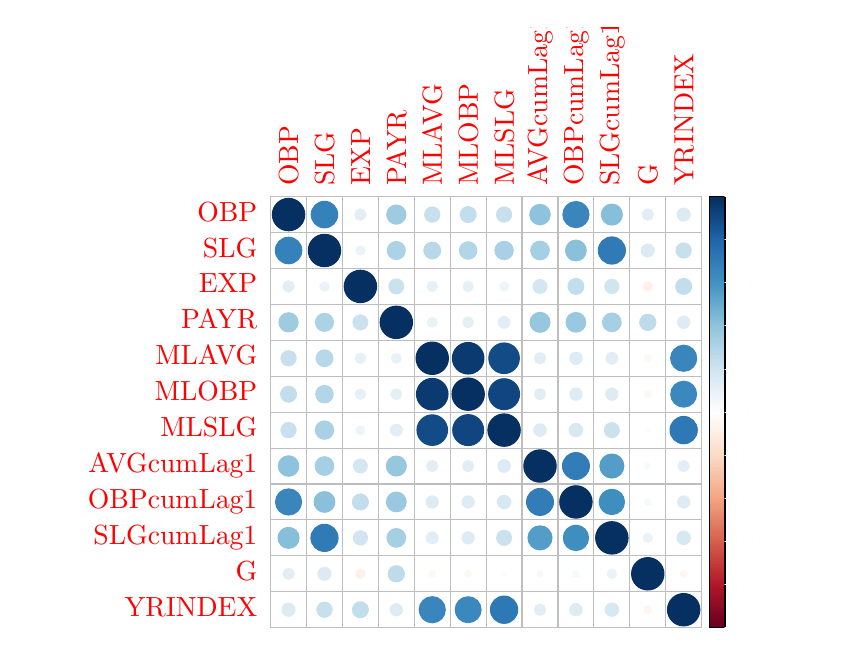
\begin{tikzpicture}[x=1pt,y=1pt]
\definecolor{fillColor}{RGB}{255,255,255}
\path[use as bounding box,fill=fillColor,fill opacity=0.00] (0,0) rectangle (289.08,216.81);
\begin{scope}
\path[clip] (  0.00,  0.00) rectangle (289.08,216.81);
\definecolor{drawColor}{RGB}{255,255,255}
\definecolor{fillColor}{RGB}{255,255,255}

\path[draw=drawColor,line width= 0.4pt,line join=round,line cap=round,fill=fillColor] ( 87.78,142.78) rectangle (100.76,155.76);

\path[draw=drawColor,line width= 0.4pt,line join=round,line cap=round,fill=fillColor] ( 87.78,129.80) rectangle (100.76,142.78);

\path[draw=drawColor,line width= 0.4pt,line join=round,line cap=round,fill=fillColor] ( 87.78,116.82) rectangle (100.76,129.80);

\path[draw=drawColor,line width= 0.4pt,line join=round,line cap=round,fill=fillColor] ( 87.78,103.84) rectangle (100.76,116.82);

\path[draw=drawColor,line width= 0.4pt,line join=round,line cap=round,fill=fillColor] ( 87.78, 90.86) rectangle (100.76,103.84);

\path[draw=drawColor,line width= 0.4pt,line join=round,line cap=round,fill=fillColor] ( 87.78, 77.88) rectangle (100.76, 90.86);

\path[draw=drawColor,line width= 0.4pt,line join=round,line cap=round,fill=fillColor] ( 87.78, 64.90) rectangle (100.76, 77.88);

\path[draw=drawColor,line width= 0.4pt,line join=round,line cap=round,fill=fillColor] ( 87.78, 51.92) rectangle (100.76, 64.90);

\path[draw=drawColor,line width= 0.4pt,line join=round,line cap=round,fill=fillColor] ( 87.78, 38.94) rectangle (100.76, 51.92);

\path[draw=drawColor,line width= 0.4pt,line join=round,line cap=round,fill=fillColor] ( 87.78, 25.96) rectangle (100.76, 38.94);

\path[draw=drawColor,line width= 0.4pt,line join=round,line cap=round,fill=fillColor] ( 87.78, 12.98) rectangle (100.76, 25.96);

\path[draw=drawColor,line width= 0.4pt,line join=round,line cap=round,fill=fillColor] ( 87.78,  0.00) rectangle (100.76, 12.98);

\path[draw=drawColor,line width= 0.4pt,line join=round,line cap=round,fill=fillColor] (100.76,142.78) rectangle (113.74,155.76);

\path[draw=drawColor,line width= 0.4pt,line join=round,line cap=round,fill=fillColor] (100.76,129.80) rectangle (113.74,142.78);

\path[draw=drawColor,line width= 0.4pt,line join=round,line cap=round,fill=fillColor] (100.76,116.82) rectangle (113.74,129.80);

\path[draw=drawColor,line width= 0.4pt,line join=round,line cap=round,fill=fillColor] (100.76,103.84) rectangle (113.74,116.82);

\path[draw=drawColor,line width= 0.4pt,line join=round,line cap=round,fill=fillColor] (100.76, 90.86) rectangle (113.74,103.84);

\path[draw=drawColor,line width= 0.4pt,line join=round,line cap=round,fill=fillColor] (100.76, 77.88) rectangle (113.74, 90.86);

\path[draw=drawColor,line width= 0.4pt,line join=round,line cap=round,fill=fillColor] (100.76, 64.90) rectangle (113.74, 77.88);

\path[draw=drawColor,line width= 0.4pt,line join=round,line cap=round,fill=fillColor] (100.76, 51.92) rectangle (113.74, 64.90);

\path[draw=drawColor,line width= 0.4pt,line join=round,line cap=round,fill=fillColor] (100.76, 38.94) rectangle (113.74, 51.92);

\path[draw=drawColor,line width= 0.4pt,line join=round,line cap=round,fill=fillColor] (100.76, 25.96) rectangle (113.74, 38.94);

\path[draw=drawColor,line width= 0.4pt,line join=round,line cap=round,fill=fillColor] (100.76, 12.98) rectangle (113.74, 25.96);

\path[draw=drawColor,line width= 0.4pt,line join=round,line cap=round,fill=fillColor] (100.76,  0.00) rectangle (113.74, 12.98);

\path[draw=drawColor,line width= 0.4pt,line join=round,line cap=round,fill=fillColor] (113.74,142.78) rectangle (126.72,155.76);

\path[draw=drawColor,line width= 0.4pt,line join=round,line cap=round,fill=fillColor] (113.74,129.80) rectangle (126.72,142.78);

\path[draw=drawColor,line width= 0.4pt,line join=round,line cap=round,fill=fillColor] (113.74,116.82) rectangle (126.72,129.80);

\path[draw=drawColor,line width= 0.4pt,line join=round,line cap=round,fill=fillColor] (113.74,103.84) rectangle (126.72,116.82);

\path[draw=drawColor,line width= 0.4pt,line join=round,line cap=round,fill=fillColor] (113.74, 90.86) rectangle (126.72,103.84);

\path[draw=drawColor,line width= 0.4pt,line join=round,line cap=round,fill=fillColor] (113.74, 77.88) rectangle (126.72, 90.86);

\path[draw=drawColor,line width= 0.4pt,line join=round,line cap=round,fill=fillColor] (113.74, 64.90) rectangle (126.72, 77.88);

\path[draw=drawColor,line width= 0.4pt,line join=round,line cap=round,fill=fillColor] (113.74, 51.92) rectangle (126.72, 64.90);

\path[draw=drawColor,line width= 0.4pt,line join=round,line cap=round,fill=fillColor] (113.74, 38.94) rectangle (126.72, 51.92);

\path[draw=drawColor,line width= 0.4pt,line join=round,line cap=round,fill=fillColor] (113.74, 25.96) rectangle (126.72, 38.94);

\path[draw=drawColor,line width= 0.4pt,line join=round,line cap=round,fill=fillColor] (113.74, 12.98) rectangle (126.72, 25.96);

\path[draw=drawColor,line width= 0.4pt,line join=round,line cap=round,fill=fillColor] (113.74,  0.00) rectangle (126.72, 12.98);

\path[draw=drawColor,line width= 0.4pt,line join=round,line cap=round,fill=fillColor] (126.72,142.78) rectangle (139.70,155.76);

\path[draw=drawColor,line width= 0.4pt,line join=round,line cap=round,fill=fillColor] (126.72,129.80) rectangle (139.70,142.78);

\path[draw=drawColor,line width= 0.4pt,line join=round,line cap=round,fill=fillColor] (126.72,116.82) rectangle (139.70,129.80);

\path[draw=drawColor,line width= 0.4pt,line join=round,line cap=round,fill=fillColor] (126.72,103.84) rectangle (139.70,116.82);

\path[draw=drawColor,line width= 0.4pt,line join=round,line cap=round,fill=fillColor] (126.72, 90.86) rectangle (139.70,103.84);

\path[draw=drawColor,line width= 0.4pt,line join=round,line cap=round,fill=fillColor] (126.72, 77.88) rectangle (139.70, 90.86);

\path[draw=drawColor,line width= 0.4pt,line join=round,line cap=round,fill=fillColor] (126.72, 64.90) rectangle (139.70, 77.88);

\path[draw=drawColor,line width= 0.4pt,line join=round,line cap=round,fill=fillColor] (126.72, 51.92) rectangle (139.70, 64.90);

\path[draw=drawColor,line width= 0.4pt,line join=round,line cap=round,fill=fillColor] (126.72, 38.94) rectangle (139.70, 51.92);

\path[draw=drawColor,line width= 0.4pt,line join=round,line cap=round,fill=fillColor] (126.72, 25.96) rectangle (139.70, 38.94);

\path[draw=drawColor,line width= 0.4pt,line join=round,line cap=round,fill=fillColor] (126.72, 12.98) rectangle (139.70, 25.96);

\path[draw=drawColor,line width= 0.4pt,line join=round,line cap=round,fill=fillColor] (126.72,  0.00) rectangle (139.70, 12.98);

\path[draw=drawColor,line width= 0.4pt,line join=round,line cap=round,fill=fillColor] (139.70,142.78) rectangle (152.68,155.76);

\path[draw=drawColor,line width= 0.4pt,line join=round,line cap=round,fill=fillColor] (139.70,129.80) rectangle (152.68,142.78);

\path[draw=drawColor,line width= 0.4pt,line join=round,line cap=round,fill=fillColor] (139.70,116.82) rectangle (152.68,129.80);

\path[draw=drawColor,line width= 0.4pt,line join=round,line cap=round,fill=fillColor] (139.70,103.84) rectangle (152.68,116.82);

\path[draw=drawColor,line width= 0.4pt,line join=round,line cap=round,fill=fillColor] (139.70, 90.86) rectangle (152.68,103.84);

\path[draw=drawColor,line width= 0.4pt,line join=round,line cap=round,fill=fillColor] (139.70, 77.88) rectangle (152.68, 90.86);

\path[draw=drawColor,line width= 0.4pt,line join=round,line cap=round,fill=fillColor] (139.70, 64.90) rectangle (152.68, 77.88);

\path[draw=drawColor,line width= 0.4pt,line join=round,line cap=round,fill=fillColor] (139.70, 51.92) rectangle (152.68, 64.90);

\path[draw=drawColor,line width= 0.4pt,line join=round,line cap=round,fill=fillColor] (139.70, 38.94) rectangle (152.68, 51.92);

\path[draw=drawColor,line width= 0.4pt,line join=round,line cap=round,fill=fillColor] (139.70, 25.96) rectangle (152.68, 38.94);

\path[draw=drawColor,line width= 0.4pt,line join=round,line cap=round,fill=fillColor] (139.70, 12.98) rectangle (152.68, 25.96);

\path[draw=drawColor,line width= 0.4pt,line join=round,line cap=round,fill=fillColor] (139.70,  0.00) rectangle (152.68, 12.98);

\path[draw=drawColor,line width= 0.4pt,line join=round,line cap=round,fill=fillColor] (152.68,142.78) rectangle (165.66,155.76);

\path[draw=drawColor,line width= 0.4pt,line join=round,line cap=round,fill=fillColor] (152.68,129.80) rectangle (165.66,142.78);

\path[draw=drawColor,line width= 0.4pt,line join=round,line cap=round,fill=fillColor] (152.68,116.82) rectangle (165.66,129.80);

\path[draw=drawColor,line width= 0.4pt,line join=round,line cap=round,fill=fillColor] (152.68,103.84) rectangle (165.66,116.82);

\path[draw=drawColor,line width= 0.4pt,line join=round,line cap=round,fill=fillColor] (152.68, 90.86) rectangle (165.66,103.84);

\path[draw=drawColor,line width= 0.4pt,line join=round,line cap=round,fill=fillColor] (152.68, 77.88) rectangle (165.66, 90.86);

\path[draw=drawColor,line width= 0.4pt,line join=round,line cap=round,fill=fillColor] (152.68, 64.90) rectangle (165.66, 77.88);

\path[draw=drawColor,line width= 0.4pt,line join=round,line cap=round,fill=fillColor] (152.68, 51.92) rectangle (165.66, 64.90);

\path[draw=drawColor,line width= 0.4pt,line join=round,line cap=round,fill=fillColor] (152.68, 38.94) rectangle (165.66, 51.92);

\path[draw=drawColor,line width= 0.4pt,line join=round,line cap=round,fill=fillColor] (152.68, 25.96) rectangle (165.66, 38.94);

\path[draw=drawColor,line width= 0.4pt,line join=round,line cap=round,fill=fillColor] (152.68, 12.98) rectangle (165.66, 25.96);

\path[draw=drawColor,line width= 0.4pt,line join=round,line cap=round,fill=fillColor] (152.68,  0.00) rectangle (165.66, 12.98);

\path[draw=drawColor,line width= 0.4pt,line join=round,line cap=round,fill=fillColor] (165.66,142.78) rectangle (178.64,155.76);

\path[draw=drawColor,line width= 0.4pt,line join=round,line cap=round,fill=fillColor] (165.66,129.80) rectangle (178.64,142.78);

\path[draw=drawColor,line width= 0.4pt,line join=round,line cap=round,fill=fillColor] (165.66,116.82) rectangle (178.64,129.80);

\path[draw=drawColor,line width= 0.4pt,line join=round,line cap=round,fill=fillColor] (165.66,103.84) rectangle (178.64,116.82);

\path[draw=drawColor,line width= 0.4pt,line join=round,line cap=round,fill=fillColor] (165.66, 90.86) rectangle (178.64,103.84);

\path[draw=drawColor,line width= 0.4pt,line join=round,line cap=round,fill=fillColor] (165.66, 77.88) rectangle (178.64, 90.86);

\path[draw=drawColor,line width= 0.4pt,line join=round,line cap=round,fill=fillColor] (165.66, 64.90) rectangle (178.64, 77.88);

\path[draw=drawColor,line width= 0.4pt,line join=round,line cap=round,fill=fillColor] (165.66, 51.92) rectangle (178.64, 64.90);

\path[draw=drawColor,line width= 0.4pt,line join=round,line cap=round,fill=fillColor] (165.66, 38.94) rectangle (178.64, 51.92);

\path[draw=drawColor,line width= 0.4pt,line join=round,line cap=round,fill=fillColor] (165.66, 25.96) rectangle (178.64, 38.94);

\path[draw=drawColor,line width= 0.4pt,line join=round,line cap=round,fill=fillColor] (165.66, 12.98) rectangle (178.64, 25.96);

\path[draw=drawColor,line width= 0.4pt,line join=round,line cap=round,fill=fillColor] (165.66,  0.00) rectangle (178.64, 12.98);

\path[draw=drawColor,line width= 0.4pt,line join=round,line cap=round,fill=fillColor] (178.64,142.78) rectangle (191.62,155.76);

\path[draw=drawColor,line width= 0.4pt,line join=round,line cap=round,fill=fillColor] (178.64,129.80) rectangle (191.62,142.78);

\path[draw=drawColor,line width= 0.4pt,line join=round,line cap=round,fill=fillColor] (178.64,116.82) rectangle (191.62,129.80);

\path[draw=drawColor,line width= 0.4pt,line join=round,line cap=round,fill=fillColor] (178.64,103.84) rectangle (191.62,116.82);

\path[draw=drawColor,line width= 0.4pt,line join=round,line cap=round,fill=fillColor] (178.64, 90.86) rectangle (191.62,103.84);

\path[draw=drawColor,line width= 0.4pt,line join=round,line cap=round,fill=fillColor] (178.64, 77.88) rectangle (191.62, 90.86);

\path[draw=drawColor,line width= 0.4pt,line join=round,line cap=round,fill=fillColor] (178.64, 64.90) rectangle (191.62, 77.88);

\path[draw=drawColor,line width= 0.4pt,line join=round,line cap=round,fill=fillColor] (178.64, 51.92) rectangle (191.62, 64.90);

\path[draw=drawColor,line width= 0.4pt,line join=round,line cap=round,fill=fillColor] (178.64, 38.94) rectangle (191.62, 51.92);

\path[draw=drawColor,line width= 0.4pt,line join=round,line cap=round,fill=fillColor] (178.64, 25.96) rectangle (191.62, 38.94);

\path[draw=drawColor,line width= 0.4pt,line join=round,line cap=round,fill=fillColor] (178.64, 12.98) rectangle (191.62, 25.96);

\path[draw=drawColor,line width= 0.4pt,line join=round,line cap=round,fill=fillColor] (178.64,  0.00) rectangle (191.62, 12.98);

\path[draw=drawColor,line width= 0.4pt,line join=round,line cap=round,fill=fillColor] (191.62,142.78) rectangle (204.60,155.76);

\path[draw=drawColor,line width= 0.4pt,line join=round,line cap=round,fill=fillColor] (191.62,129.80) rectangle (204.60,142.78);

\path[draw=drawColor,line width= 0.4pt,line join=round,line cap=round,fill=fillColor] (191.62,116.82) rectangle (204.60,129.80);

\path[draw=drawColor,line width= 0.4pt,line join=round,line cap=round,fill=fillColor] (191.62,103.84) rectangle (204.60,116.82);

\path[draw=drawColor,line width= 0.4pt,line join=round,line cap=round,fill=fillColor] (191.62, 90.86) rectangle (204.60,103.84);

\path[draw=drawColor,line width= 0.4pt,line join=round,line cap=round,fill=fillColor] (191.62, 77.88) rectangle (204.60, 90.86);

\path[draw=drawColor,line width= 0.4pt,line join=round,line cap=round,fill=fillColor] (191.62, 64.90) rectangle (204.60, 77.88);

\path[draw=drawColor,line width= 0.4pt,line join=round,line cap=round,fill=fillColor] (191.62, 51.92) rectangle (204.60, 64.90);

\path[draw=drawColor,line width= 0.4pt,line join=round,line cap=round,fill=fillColor] (191.62, 38.94) rectangle (204.60, 51.92);

\path[draw=drawColor,line width= 0.4pt,line join=round,line cap=round,fill=fillColor] (191.62, 25.96) rectangle (204.60, 38.94);

\path[draw=drawColor,line width= 0.4pt,line join=round,line cap=round,fill=fillColor] (191.62, 12.98) rectangle (204.60, 25.96);

\path[draw=drawColor,line width= 0.4pt,line join=round,line cap=round,fill=fillColor] (191.62,  0.00) rectangle (204.60, 12.98);

\path[draw=drawColor,line width= 0.4pt,line join=round,line cap=round,fill=fillColor] (204.60,142.78) rectangle (217.58,155.76);

\path[draw=drawColor,line width= 0.4pt,line join=round,line cap=round,fill=fillColor] (204.60,129.80) rectangle (217.58,142.78);

\path[draw=drawColor,line width= 0.4pt,line join=round,line cap=round,fill=fillColor] (204.60,116.82) rectangle (217.58,129.80);

\path[draw=drawColor,line width= 0.4pt,line join=round,line cap=round,fill=fillColor] (204.60,103.84) rectangle (217.58,116.82);

\path[draw=drawColor,line width= 0.4pt,line join=round,line cap=round,fill=fillColor] (204.60, 90.86) rectangle (217.58,103.84);

\path[draw=drawColor,line width= 0.4pt,line join=round,line cap=round,fill=fillColor] (204.60, 77.88) rectangle (217.58, 90.86);

\path[draw=drawColor,line width= 0.4pt,line join=round,line cap=round,fill=fillColor] (204.60, 64.90) rectangle (217.58, 77.88);

\path[draw=drawColor,line width= 0.4pt,line join=round,line cap=round,fill=fillColor] (204.60, 51.92) rectangle (217.58, 64.90);

\path[draw=drawColor,line width= 0.4pt,line join=round,line cap=round,fill=fillColor] (204.60, 38.94) rectangle (217.58, 51.92);

\path[draw=drawColor,line width= 0.4pt,line join=round,line cap=round,fill=fillColor] (204.60, 25.96) rectangle (217.58, 38.94);

\path[draw=drawColor,line width= 0.4pt,line join=round,line cap=round,fill=fillColor] (204.60, 12.98) rectangle (217.58, 25.96);

\path[draw=drawColor,line width= 0.4pt,line join=round,line cap=round,fill=fillColor] (204.60,  0.00) rectangle (217.58, 12.98);

\path[draw=drawColor,line width= 0.4pt,line join=round,line cap=round,fill=fillColor] (217.58,142.78) rectangle (230.56,155.76);

\path[draw=drawColor,line width= 0.4pt,line join=round,line cap=round,fill=fillColor] (217.58,129.80) rectangle (230.56,142.78);

\path[draw=drawColor,line width= 0.4pt,line join=round,line cap=round,fill=fillColor] (217.58,116.82) rectangle (230.56,129.80);

\path[draw=drawColor,line width= 0.4pt,line join=round,line cap=round,fill=fillColor] (217.58,103.84) rectangle (230.56,116.82);

\path[draw=drawColor,line width= 0.4pt,line join=round,line cap=round,fill=fillColor] (217.58, 90.86) rectangle (230.56,103.84);

\path[draw=drawColor,line width= 0.4pt,line join=round,line cap=round,fill=fillColor] (217.58, 77.88) rectangle (230.56, 90.86);

\path[draw=drawColor,line width= 0.4pt,line join=round,line cap=round,fill=fillColor] (217.58, 64.90) rectangle (230.56, 77.88);

\path[draw=drawColor,line width= 0.4pt,line join=round,line cap=round,fill=fillColor] (217.58, 51.92) rectangle (230.56, 64.90);

\path[draw=drawColor,line width= 0.4pt,line join=round,line cap=round,fill=fillColor] (217.58, 38.94) rectangle (230.56, 51.92);

\path[draw=drawColor,line width= 0.4pt,line join=round,line cap=round,fill=fillColor] (217.58, 25.96) rectangle (230.56, 38.94);

\path[draw=drawColor,line width= 0.4pt,line join=round,line cap=round,fill=fillColor] (217.58, 12.98) rectangle (230.56, 25.96);

\path[draw=drawColor,line width= 0.4pt,line join=round,line cap=round,fill=fillColor] (217.58,  0.00) rectangle (230.56, 12.98);

\path[draw=drawColor,line width= 0.4pt,line join=round,line cap=round,fill=fillColor] (230.56,142.78) rectangle (243.53,155.76);

\path[draw=drawColor,line width= 0.4pt,line join=round,line cap=round,fill=fillColor] (230.56,129.80) rectangle (243.53,142.78);

\path[draw=drawColor,line width= 0.4pt,line join=round,line cap=round,fill=fillColor] (230.56,116.82) rectangle (243.53,129.80);

\path[draw=drawColor,line width= 0.4pt,line join=round,line cap=round,fill=fillColor] (230.56,103.84) rectangle (243.53,116.82);

\path[draw=drawColor,line width= 0.4pt,line join=round,line cap=round,fill=fillColor] (230.56, 90.86) rectangle (243.53,103.84);

\path[draw=drawColor,line width= 0.4pt,line join=round,line cap=round,fill=fillColor] (230.56, 77.88) rectangle (243.53, 90.86);

\path[draw=drawColor,line width= 0.4pt,line join=round,line cap=round,fill=fillColor] (230.56, 64.90) rectangle (243.53, 77.88);

\path[draw=drawColor,line width= 0.4pt,line join=round,line cap=round,fill=fillColor] (230.56, 51.92) rectangle (243.53, 64.90);

\path[draw=drawColor,line width= 0.4pt,line join=round,line cap=round,fill=fillColor] (230.56, 38.94) rectangle (243.53, 51.92);

\path[draw=drawColor,line width= 0.4pt,line join=round,line cap=round,fill=fillColor] (230.56, 25.96) rectangle (243.53, 38.94);

\path[draw=drawColor,line width= 0.4pt,line join=round,line cap=round,fill=fillColor] (230.56, 12.98) rectangle (243.53, 25.96);

\path[draw=drawColor,line width= 0.4pt,line join=round,line cap=round,fill=fillColor] (230.56,  0.00) rectangle (243.53, 12.98);
\definecolor{drawColor}{RGB}{5,48,97}
\definecolor{fillColor}{RGB}{5,48,97}

\path[draw=drawColor,line width= 0.4pt,line join=round,line cap=round,fill=fillColor] ( 94.27,149.27) circle (  5.84);
\definecolor{drawColor}{RGB}{53,129,185}
\definecolor{fillColor}{RGB}{53,129,185}

\path[draw=drawColor,line width= 0.4pt,line join=round,line cap=round,fill=fillColor] ( 94.27,136.29) circle (  4.78);
\definecolor{drawColor}{RGB}{226,238,245}
\definecolor{fillColor}{RGB}{226,238,245}

\path[draw=drawColor,line width= 0.4pt,line join=round,line cap=round,fill=fillColor] ( 94.27,123.31) circle (  2.02);
\definecolor{drawColor}{RGB}{159,203,225}
\definecolor{fillColor}{RGB}{159,203,225}

\path[draw=drawColor,line width= 0.4pt,line join=round,line cap=round,fill=fillColor] ( 94.27,110.33) circle (  3.46);
\definecolor{drawColor}{RGB}{200,224,237}
\definecolor{fillColor}{RGB}{200,224,237}

\path[draw=drawColor,line width= 0.4pt,line join=round,line cap=round,fill=fillColor] ( 94.27, 97.35) circle (  2.74);
\definecolor{drawColor}{RGB}{194,221,235}
\definecolor{fillColor}{RGB}{194,221,235}

\path[draw=drawColor,line width= 0.4pt,line join=round,line cap=round,fill=fillColor] ( 94.27, 84.37) circle (  2.86);
\definecolor{drawColor}{RGB}{200,224,237}
\definecolor{fillColor}{RGB}{200,224,237}

\path[draw=drawColor,line width= 0.4pt,line join=round,line cap=round,fill=fillColor] ( 94.27, 71.39) circle (  2.74);
\definecolor{drawColor}{RGB}{143,195,221}
\definecolor{fillColor}{RGB}{143,195,221}

\path[draw=drawColor,line width= 0.4pt,line join=round,line cap=round,fill=fillColor] ( 94.27, 58.41) circle (  3.69);
\definecolor{drawColor}{RGB}{57,133,188}
\definecolor{fillColor}{RGB}{57,133,188}

\path[draw=drawColor,line width= 0.4pt,line join=round,line cap=round,fill=fillColor] ( 94.27, 45.43) circle (  4.71);
\definecolor{drawColor}{RGB}{135,190,218}
\definecolor{fillColor}{RGB}{135,190,218}

\path[draw=drawColor,line width= 0.4pt,line join=round,line cap=round,fill=fillColor] ( 94.27, 32.45) circle (  3.79);
\definecolor{drawColor}{RGB}{226,238,245}
\definecolor{fillColor}{RGB}{226,238,245}

\path[draw=drawColor,line width= 0.4pt,line join=round,line cap=round,fill=fillColor] ( 94.27, 19.47) circle (  2.02);
\definecolor{drawColor}{RGB}{219,234,243}
\definecolor{fillColor}{RGB}{219,234,243}

\path[draw=drawColor,line width= 0.4pt,line join=round,line cap=round,fill=fillColor] ( 94.27,  6.49) circle (  2.34);
\definecolor{drawColor}{RGB}{53,129,185}
\definecolor{fillColor}{RGB}{53,129,185}

\path[draw=drawColor,line width= 0.4pt,line join=round,line cap=round,fill=fillColor] (107.25,149.27) circle (  4.78);
\definecolor{drawColor}{RGB}{5,48,97}
\definecolor{fillColor}{RGB}{5,48,97}

\path[draw=drawColor,line width= 0.4pt,line join=round,line cap=round,fill=fillColor] (107.25,136.29) circle (  5.84);
\definecolor{drawColor}{RGB}{235,243,248}
\definecolor{fillColor}{RGB}{235,243,248}

\path[draw=drawColor,line width= 0.4pt,line join=round,line cap=round,fill=fillColor] (107.25,123.31) circle (  1.65);
\definecolor{drawColor}{RGB}{172,210,229}
\definecolor{fillColor}{RGB}{172,210,229}

\path[draw=drawColor,line width= 0.4pt,line join=round,line cap=round,fill=fillColor] (107.25,110.33) circle (  3.25);
\definecolor{drawColor}{RGB}{184,216,233}
\definecolor{fillColor}{RGB}{184,216,233}

\path[draw=drawColor,line width= 0.4pt,line join=round,line cap=round,fill=fillColor] (107.25, 97.35) circle (  3.03);
\definecolor{drawColor}{RGB}{178,213,231}
\definecolor{fillColor}{RGB}{178,213,231}

\path[draw=drawColor,line width= 0.4pt,line join=round,line cap=round,fill=fillColor] (107.25, 84.37) circle (  3.15);
\definecolor{drawColor}{RGB}{169,208,228}
\definecolor{fillColor}{RGB}{169,208,228}

\path[draw=drawColor,line width= 0.4pt,line join=round,line cap=round,fill=fillColor] (107.25, 71.39) circle (  3.30);
\definecolor{drawColor}{RGB}{165,207,227}
\definecolor{fillColor}{RGB}{165,207,227}

\path[draw=drawColor,line width= 0.4pt,line join=round,line cap=round,fill=fillColor] (107.25, 58.41) circle (  3.36);
\definecolor{drawColor}{RGB}{139,192,219}
\definecolor{fillColor}{RGB}{139,192,219}

\path[draw=drawColor,line width= 0.4pt,line join=round,line cap=round,fill=fillColor] (107.25, 45.43) circle (  3.74);
\definecolor{drawColor}{RGB}{48,122,182}
\definecolor{fillColor}{RGB}{48,122,182}

\path[draw=drawColor,line width= 0.4pt,line join=round,line cap=round,fill=fillColor] (107.25, 32.45) circle (  4.89);
\definecolor{drawColor}{RGB}{219,234,243}
\definecolor{fillColor}{RGB}{219,234,243}

\path[draw=drawColor,line width= 0.4pt,line join=round,line cap=round,fill=fillColor] (107.25, 19.47) circle (  2.34);
\definecolor{drawColor}{RGB}{200,224,237}
\definecolor{fillColor}{RGB}{200,224,237}

\path[draw=drawColor,line width= 0.4pt,line join=round,line cap=round,fill=fillColor] (107.25,  6.49) circle (  2.74);
\definecolor{drawColor}{RGB}{226,238,245}
\definecolor{fillColor}{RGB}{226,238,245}

\path[draw=drawColor,line width= 0.4pt,line join=round,line cap=round,fill=fillColor] (120.23,149.27) circle (  2.02);
\definecolor{drawColor}{RGB}{235,243,248}
\definecolor{fillColor}{RGB}{235,243,248}

\path[draw=drawColor,line width= 0.4pt,line join=round,line cap=round,fill=fillColor] (120.23,136.29) circle (  1.65);
\definecolor{drawColor}{RGB}{5,48,97}
\definecolor{fillColor}{RGB}{5,48,97}

\path[draw=drawColor,line width= 0.4pt,line join=round,line cap=round,fill=fillColor] (120.23,123.31) circle (  5.84);
\definecolor{drawColor}{RGB}{203,226,238}
\definecolor{fillColor}{RGB}{203,226,238}

\path[draw=drawColor,line width= 0.4pt,line join=round,line cap=round,fill=fillColor] (120.23,110.33) circle (  2.68);
\definecolor{drawColor}{RGB}{230,241,247}
\definecolor{fillColor}{RGB}{230,241,247}

\path[draw=drawColor,line width= 0.4pt,line join=round,line cap=round,fill=fillColor] (120.23, 97.35) circle (  1.85);

\path[draw=drawColor,line width= 0.4pt,line join=round,line cap=round,fill=fillColor] (120.23, 84.37) circle (  1.85);
\definecolor{drawColor}{RGB}{237,245,249}
\definecolor{fillColor}{RGB}{237,245,249}

\path[draw=drawColor,line width= 0.4pt,line join=round,line cap=round,fill=fillColor] (120.23, 71.39) circle (  1.55);
\definecolor{drawColor}{RGB}{212,230,241}
\definecolor{fillColor}{RGB}{212,230,241}

\path[draw=drawColor,line width= 0.4pt,line join=round,line cap=round,fill=fillColor] (120.23, 58.41) circle (  2.48);
\definecolor{drawColor}{RGB}{194,221,235}
\definecolor{fillColor}{RGB}{194,221,235}

\path[draw=drawColor,line width= 0.4pt,line join=round,line cap=round,fill=fillColor] (120.23, 45.43) circle (  2.86);
\definecolor{drawColor}{RGB}{209,229,240}
\definecolor{fillColor}{RGB}{209,229,240}

\path[draw=drawColor,line width= 0.4pt,line join=round,line cap=round,fill=fillColor] (120.23, 32.45) circle (  2.55);
\definecolor{drawColor}{RGB}{254,241,233}
\definecolor{fillColor}{RGB}{254,241,233}

\path[draw=drawColor,line width= 0.4pt,line join=round,line cap=round,fill=fillColor] (120.23, 19.47) circle (  1.65);
\definecolor{drawColor}{RGB}{194,221,235}
\definecolor{fillColor}{RGB}{194,221,235}

\path[draw=drawColor,line width= 0.4pt,line join=round,line cap=round,fill=fillColor] (120.23,  6.49) circle (  2.86);
\definecolor{drawColor}{RGB}{159,203,225}
\definecolor{fillColor}{RGB}{159,203,225}

\path[draw=drawColor,line width= 0.4pt,line join=round,line cap=round,fill=fillColor] (133.21,149.27) circle (  3.46);
\definecolor{drawColor}{RGB}{172,210,229}
\definecolor{fillColor}{RGB}{172,210,229}

\path[draw=drawColor,line width= 0.4pt,line join=round,line cap=round,fill=fillColor] (133.21,136.29) circle (  3.25);
\definecolor{drawColor}{RGB}{203,226,238}
\definecolor{fillColor}{RGB}{203,226,238}

\path[draw=drawColor,line width= 0.4pt,line join=round,line cap=round,fill=fillColor] (133.21,123.31) circle (  2.68);
\definecolor{drawColor}{RGB}{5,48,97}
\definecolor{fillColor}{RGB}{5,48,97}

\path[draw=drawColor,line width= 0.4pt,line join=round,line cap=round,fill=fillColor] (133.21,110.33) circle (  5.84);
\definecolor{drawColor}{RGB}{233,242,247}
\definecolor{fillColor}{RGB}{233,242,247}

\path[draw=drawColor,line width= 0.4pt,line join=round,line cap=round,fill=fillColor] (133.21, 97.35) circle (  1.75);
\definecolor{drawColor}{RGB}{228,239,246}
\definecolor{fillColor}{RGB}{228,239,246}

\path[draw=drawColor,line width= 0.4pt,line join=round,line cap=round,fill=fillColor] (133.21, 84.37) circle (  1.94);
\definecolor{drawColor}{RGB}{226,238,245}
\definecolor{fillColor}{RGB}{226,238,245}

\path[draw=drawColor,line width= 0.4pt,line join=round,line cap=round,fill=fillColor] (133.21, 71.39) circle (  2.11);
\definecolor{drawColor}{RGB}{150,199,223}
\definecolor{fillColor}{RGB}{150,199,223}

\path[draw=drawColor,line width= 0.4pt,line join=round,line cap=round,fill=fillColor] (133.21, 58.41) circle (  3.60);
\definecolor{drawColor}{RGB}{153,200,224}
\definecolor{fillColor}{RGB}{153,200,224}

\path[draw=drawColor,line width= 0.4pt,line join=round,line cap=round,fill=fillColor] (133.21, 45.43) circle (  3.55);
\definecolor{drawColor}{RGB}{165,207,227}
\definecolor{fillColor}{RGB}{165,207,227}

\path[draw=drawColor,line width= 0.4pt,line join=round,line cap=round,fill=fillColor] (133.21, 32.45) circle (  3.36);
\definecolor{drawColor}{RGB}{191,219,234}
\definecolor{fillColor}{RGB}{191,219,234}

\path[draw=drawColor,line width= 0.4pt,line join=round,line cap=round,fill=fillColor] (133.21, 19.47) circle (  2.92);
\definecolor{drawColor}{RGB}{221,236,244}
\definecolor{fillColor}{RGB}{221,236,244}

\path[draw=drawColor,line width= 0.4pt,line join=round,line cap=round,fill=fillColor] (133.21,  6.49) circle (  2.19);
\definecolor{drawColor}{RGB}{200,224,237}
\definecolor{fillColor}{RGB}{200,224,237}

\path[draw=drawColor,line width= 0.4pt,line join=round,line cap=round,fill=fillColor] (146.19,149.27) circle (  2.74);
\definecolor{drawColor}{RGB}{184,216,233}
\definecolor{fillColor}{RGB}{184,216,233}

\path[draw=drawColor,line width= 0.4pt,line join=round,line cap=round,fill=fillColor] (146.19,136.29) circle (  3.03);
\definecolor{drawColor}{RGB}{230,241,247}
\definecolor{fillColor}{RGB}{230,241,247}

\path[draw=drawColor,line width= 0.4pt,line join=round,line cap=round,fill=fillColor] (146.19,123.31) circle (  1.85);
\definecolor{drawColor}{RGB}{233,242,247}
\definecolor{fillColor}{RGB}{233,242,247}

\path[draw=drawColor,line width= 0.4pt,line join=round,line cap=round,fill=fillColor] (146.19,110.33) circle (  1.75);
\definecolor{drawColor}{RGB}{5,48,97}
\definecolor{fillColor}{RGB}{5,48,97}

\path[draw=drawColor,line width= 0.4pt,line join=round,line cap=round,fill=fillColor] (146.19, 97.35) circle (  5.84);
\definecolor{drawColor}{RGB}{10,58,112}
\definecolor{fillColor}{RGB}{10,58,112}

\path[draw=drawColor,line width= 0.4pt,line join=round,line cap=round,fill=fillColor] (146.19, 84.37) circle (  5.69);
\definecolor{drawColor}{RGB}{19,75,134}
\definecolor{fillColor}{RGB}{19,75,134}

\path[draw=drawColor,line width= 0.4pt,line join=round,line cap=round,fill=fillColor] (146.19, 71.39) circle (  5.51);
\definecolor{drawColor}{RGB}{226,238,245}
\definecolor{fillColor}{RGB}{226,238,245}

\path[draw=drawColor,line width= 0.4pt,line join=round,line cap=round,fill=fillColor] (146.19, 58.41) circle (  2.02);
\definecolor{drawColor}{RGB}{221,236,244}
\definecolor{fillColor}{RGB}{221,236,244}

\path[draw=drawColor,line width= 0.4pt,line join=round,line cap=round,fill=fillColor] (146.19, 45.43) circle (  2.19);
\definecolor{drawColor}{RGB}{226,238,245}
\definecolor{fillColor}{RGB}{226,238,245}

\path[draw=drawColor,line width= 0.4pt,line join=round,line cap=round,fill=fillColor] (146.19, 32.45) circle (  2.11);
\definecolor{drawColor}{RGB}{254,248,245}
\definecolor{fillColor}{RGB}{254,248,245}

\path[draw=drawColor,line width= 0.4pt,line join=round,line cap=round,fill=fillColor] (146.19, 19.47) circle (  1.17);
\definecolor{drawColor}{RGB}{57,133,188}
\definecolor{fillColor}{RGB}{57,133,188}

\path[draw=drawColor,line width= 0.4pt,line join=round,line cap=round,fill=fillColor] (146.19,  6.49) circle (  4.71);
\definecolor{drawColor}{RGB}{194,221,235}
\definecolor{fillColor}{RGB}{194,221,235}

\path[draw=drawColor,line width= 0.4pt,line join=round,line cap=round,fill=fillColor] (159.17,149.27) circle (  2.86);
\definecolor{drawColor}{RGB}{178,213,231}
\definecolor{fillColor}{RGB}{178,213,231}

\path[draw=drawColor,line width= 0.4pt,line join=round,line cap=round,fill=fillColor] (159.17,136.29) circle (  3.15);
\definecolor{drawColor}{RGB}{230,241,247}
\definecolor{fillColor}{RGB}{230,241,247}

\path[draw=drawColor,line width= 0.4pt,line join=round,line cap=round,fill=fillColor] (159.17,123.31) circle (  1.85);
\definecolor{drawColor}{RGB}{228,239,246}
\definecolor{fillColor}{RGB}{228,239,246}

\path[draw=drawColor,line width= 0.4pt,line join=round,line cap=round,fill=fillColor] (159.17,110.33) circle (  1.94);
\definecolor{drawColor}{RGB}{10,58,112}
\definecolor{fillColor}{RGB}{10,58,112}

\path[draw=drawColor,line width= 0.4pt,line join=round,line cap=round,fill=fillColor] (159.17, 97.35) circle (  5.69);
\definecolor{drawColor}{RGB}{5,48,97}
\definecolor{fillColor}{RGB}{5,48,97}

\path[draw=drawColor,line width= 0.4pt,line join=round,line cap=round,fill=fillColor] (159.17, 84.37) circle (  5.84);
\definecolor{drawColor}{RGB}{16,69,127}
\definecolor{fillColor}{RGB}{16,69,127}

\path[draw=drawColor,line width= 0.4pt,line join=round,line cap=round,fill=fillColor] (159.17, 71.39) circle (  5.57);
\definecolor{drawColor}{RGB}{226,238,245}
\definecolor{fillColor}{RGB}{226,238,245}

\path[draw=drawColor,line width= 0.4pt,line join=round,line cap=round,fill=fillColor] (159.17, 58.41) circle (  2.02);
\definecolor{drawColor}{RGB}{221,236,244}
\definecolor{fillColor}{RGB}{221,236,244}

\path[draw=drawColor,line width= 0.4pt,line join=round,line cap=round,fill=fillColor] (159.17, 45.43) circle (  2.19);

\path[draw=drawColor,line width= 0.4pt,line join=round,line cap=round,fill=fillColor] (159.17, 32.45) circle (  2.19);
\definecolor{drawColor}{RGB}{254,248,245}
\definecolor{fillColor}{RGB}{254,248,245}

\path[draw=drawColor,line width= 0.4pt,line join=round,line cap=round,fill=fillColor] (159.17, 19.47) circle (  1.17);
\definecolor{drawColor}{RGB}{58,136,189}
\definecolor{fillColor}{RGB}{58,136,189}

\path[draw=drawColor,line width= 0.4pt,line join=round,line cap=round,fill=fillColor] (159.17,  6.49) circle (  4.67);
\definecolor{drawColor}{RGB}{200,224,237}
\definecolor{fillColor}{RGB}{200,224,237}

\path[draw=drawColor,line width= 0.4pt,line join=round,line cap=round,fill=fillColor] (172.15,149.27) circle (  2.74);
\definecolor{drawColor}{RGB}{169,208,228}
\definecolor{fillColor}{RGB}{169,208,228}

\path[draw=drawColor,line width= 0.4pt,line join=round,line cap=round,fill=fillColor] (172.15,136.29) circle (  3.30);
\definecolor{drawColor}{RGB}{237,245,249}
\definecolor{fillColor}{RGB}{237,245,249}

\path[draw=drawColor,line width= 0.4pt,line join=round,line cap=round,fill=fillColor] (172.15,123.31) circle (  1.55);
\definecolor{drawColor}{RGB}{226,238,245}
\definecolor{fillColor}{RGB}{226,238,245}

\path[draw=drawColor,line width= 0.4pt,line join=round,line cap=round,fill=fillColor] (172.15,110.33) circle (  2.11);
\definecolor{drawColor}{RGB}{19,75,134}
\definecolor{fillColor}{RGB}{19,75,134}

\path[draw=drawColor,line width= 0.4pt,line join=round,line cap=round,fill=fillColor] (172.15, 97.35) circle (  5.51);
\definecolor{drawColor}{RGB}{16,69,127}
\definecolor{fillColor}{RGB}{16,69,127}

\path[draw=drawColor,line width= 0.4pt,line join=round,line cap=round,fill=fillColor] (172.15, 84.37) circle (  5.57);
\definecolor{drawColor}{RGB}{5,48,97}
\definecolor{fillColor}{RGB}{5,48,97}

\path[draw=drawColor,line width= 0.4pt,line join=round,line cap=round,fill=fillColor] (172.15, 71.39) circle (  5.84);
\definecolor{drawColor}{RGB}{221,236,244}
\definecolor{fillColor}{RGB}{221,236,244}

\path[draw=drawColor,line width= 0.4pt,line join=round,line cap=round,fill=fillColor] (172.15, 58.41) circle (  2.26);
\definecolor{drawColor}{RGB}{214,232,241}
\definecolor{fillColor}{RGB}{214,232,241}

\path[draw=drawColor,line width= 0.4pt,line join=round,line cap=round,fill=fillColor] (172.15, 45.43) circle (  2.41);
\definecolor{drawColor}{RGB}{203,226,238}
\definecolor{fillColor}{RGB}{203,226,238}

\path[draw=drawColor,line width= 0.4pt,line join=round,line cap=round,fill=fillColor] (172.15, 32.45) circle (  2.68);
\definecolor{drawColor}{RGB}{254,252,250}
\definecolor{fillColor}{RGB}{254,252,250}

\path[draw=drawColor,line width= 0.4pt,line join=round,line cap=round,fill=fillColor] (172.15, 19.47) circle (  0.83);
\definecolor{drawColor}{RGB}{46,120,181}
\definecolor{fillColor}{RGB}{46,120,181}

\path[draw=drawColor,line width= 0.4pt,line join=round,line cap=round,fill=fillColor] (172.15,  6.49) circle (  4.92);
\definecolor{drawColor}{RGB}{143,195,221}
\definecolor{fillColor}{RGB}{143,195,221}

\path[draw=drawColor,line width= 0.4pt,line join=round,line cap=round,fill=fillColor] (185.13,149.27) circle (  3.69);
\definecolor{drawColor}{RGB}{165,207,227}
\definecolor{fillColor}{RGB}{165,207,227}

\path[draw=drawColor,line width= 0.4pt,line join=round,line cap=round,fill=fillColor] (185.13,136.29) circle (  3.36);
\definecolor{drawColor}{RGB}{212,230,241}
\definecolor{fillColor}{RGB}{212,230,241}

\path[draw=drawColor,line width= 0.4pt,line join=round,line cap=round,fill=fillColor] (185.13,123.31) circle (  2.48);
\definecolor{drawColor}{RGB}{150,199,223}
\definecolor{fillColor}{RGB}{150,199,223}

\path[draw=drawColor,line width= 0.4pt,line join=round,line cap=round,fill=fillColor] (185.13,110.33) circle (  3.60);
\definecolor{drawColor}{RGB}{226,238,245}
\definecolor{fillColor}{RGB}{226,238,245}

\path[draw=drawColor,line width= 0.4pt,line join=round,line cap=round,fill=fillColor] (185.13, 97.35) circle (  2.02);

\path[draw=drawColor,line width= 0.4pt,line join=round,line cap=round,fill=fillColor] (185.13, 84.37) circle (  2.02);
\definecolor{drawColor}{RGB}{221,236,244}
\definecolor{fillColor}{RGB}{221,236,244}

\path[draw=drawColor,line width= 0.4pt,line join=round,line cap=round,fill=fillColor] (185.13, 71.39) circle (  2.26);
\definecolor{drawColor}{RGB}{5,48,97}
\definecolor{fillColor}{RGB}{5,48,97}

\path[draw=drawColor,line width= 0.4pt,line join=round,line cap=round,fill=fillColor] (185.13, 58.41) circle (  5.84);
\definecolor{drawColor}{RGB}{50,124,183}
\definecolor{fillColor}{RGB}{50,124,183}

\path[draw=drawColor,line width= 0.4pt,line join=round,line cap=round,fill=fillColor] (185.13, 45.43) circle (  4.85);
\definecolor{drawColor}{RGB}{83,157,200}
\definecolor{fillColor}{RGB}{83,157,200}

\path[draw=drawColor,line width= 0.4pt,line join=round,line cap=round,fill=fillColor] (185.13, 32.45) circle (  4.33);
\definecolor{drawColor}{RGB}{246,250,252}
\definecolor{fillColor}{RGB}{246,250,252}

\path[draw=drawColor,line width= 0.4pt,line join=round,line cap=round,fill=fillColor] (185.13, 19.47) circle (  1.01);
\definecolor{drawColor}{RGB}{226,238,245}
\definecolor{fillColor}{RGB}{226,238,245}

\path[draw=drawColor,line width= 0.4pt,line join=round,line cap=round,fill=fillColor] (185.13,  6.49) circle (  2.02);
\definecolor{drawColor}{RGB}{57,133,188}
\definecolor{fillColor}{RGB}{57,133,188}

\path[draw=drawColor,line width= 0.4pt,line join=round,line cap=round,fill=fillColor] (198.11,149.27) circle (  4.71);
\definecolor{drawColor}{RGB}{139,192,219}
\definecolor{fillColor}{RGB}{139,192,219}

\path[draw=drawColor,line width= 0.4pt,line join=round,line cap=round,fill=fillColor] (198.11,136.29) circle (  3.74);
\definecolor{drawColor}{RGB}{194,221,235}
\definecolor{fillColor}{RGB}{194,221,235}

\path[draw=drawColor,line width= 0.4pt,line join=round,line cap=round,fill=fillColor] (198.11,123.31) circle (  2.86);
\definecolor{drawColor}{RGB}{153,200,224}
\definecolor{fillColor}{RGB}{153,200,224}

\path[draw=drawColor,line width= 0.4pt,line join=round,line cap=round,fill=fillColor] (198.11,110.33) circle (  3.55);
\definecolor{drawColor}{RGB}{221,236,244}
\definecolor{fillColor}{RGB}{221,236,244}

\path[draw=drawColor,line width= 0.4pt,line join=round,line cap=round,fill=fillColor] (198.11, 97.35) circle (  2.19);

\path[draw=drawColor,line width= 0.4pt,line join=round,line cap=round,fill=fillColor] (198.11, 84.37) circle (  2.19);
\definecolor{drawColor}{RGB}{214,232,241}
\definecolor{fillColor}{RGB}{214,232,241}

\path[draw=drawColor,line width= 0.4pt,line join=round,line cap=round,fill=fillColor] (198.11, 71.39) circle (  2.41);
\definecolor{drawColor}{RGB}{50,124,183}
\definecolor{fillColor}{RGB}{50,124,183}

\path[draw=drawColor,line width= 0.4pt,line join=round,line cap=round,fill=fillColor] (198.11, 58.41) circle (  4.85);
\definecolor{drawColor}{RGB}{5,48,97}
\definecolor{fillColor}{RGB}{5,48,97}

\path[draw=drawColor,line width= 0.4pt,line join=round,line cap=round,fill=fillColor] (198.11, 45.43) circle (  5.84);
\definecolor{drawColor}{RGB}{63,142,192}
\definecolor{fillColor}{RGB}{63,142,192}

\path[draw=drawColor,line width= 0.4pt,line join=round,line cap=round,fill=fillColor] (198.11, 32.45) circle (  4.56);
\definecolor{drawColor}{RGB}{244,249,251}
\definecolor{fillColor}{RGB}{244,249,251}

\path[draw=drawColor,line width= 0.4pt,line join=round,line cap=round,fill=fillColor] (198.11, 19.47) circle (  1.17);
\definecolor{drawColor}{RGB}{221,236,244}
\definecolor{fillColor}{RGB}{221,236,244}

\path[draw=drawColor,line width= 0.4pt,line join=round,line cap=round,fill=fillColor] (198.11,  6.49) circle (  2.19);
\definecolor{drawColor}{RGB}{135,190,218}
\definecolor{fillColor}{RGB}{135,190,218}

\path[draw=drawColor,line width= 0.4pt,line join=round,line cap=round,fill=fillColor] (211.09,149.27) circle (  3.79);
\definecolor{drawColor}{RGB}{48,122,182}
\definecolor{fillColor}{RGB}{48,122,182}

\path[draw=drawColor,line width= 0.4pt,line join=round,line cap=round,fill=fillColor] (211.09,136.29) circle (  4.89);
\definecolor{drawColor}{RGB}{209,229,240}
\definecolor{fillColor}{RGB}{209,229,240}

\path[draw=drawColor,line width= 0.4pt,line join=round,line cap=round,fill=fillColor] (211.09,123.31) circle (  2.55);
\definecolor{drawColor}{RGB}{165,207,227}
\definecolor{fillColor}{RGB}{165,207,227}

\path[draw=drawColor,line width= 0.4pt,line join=round,line cap=round,fill=fillColor] (211.09,110.33) circle (  3.36);
\definecolor{drawColor}{RGB}{226,238,245}
\definecolor{fillColor}{RGB}{226,238,245}

\path[draw=drawColor,line width= 0.4pt,line join=round,line cap=round,fill=fillColor] (211.09, 97.35) circle (  2.11);
\definecolor{drawColor}{RGB}{221,236,244}
\definecolor{fillColor}{RGB}{221,236,244}

\path[draw=drawColor,line width= 0.4pt,line join=round,line cap=round,fill=fillColor] (211.09, 84.37) circle (  2.19);
\definecolor{drawColor}{RGB}{203,226,238}
\definecolor{fillColor}{RGB}{203,226,238}

\path[draw=drawColor,line width= 0.4pt,line join=round,line cap=round,fill=fillColor] (211.09, 71.39) circle (  2.68);
\definecolor{drawColor}{RGB}{83,157,200}
\definecolor{fillColor}{RGB}{83,157,200}

\path[draw=drawColor,line width= 0.4pt,line join=round,line cap=round,fill=fillColor] (211.09, 58.41) circle (  4.33);
\definecolor{drawColor}{RGB}{63,142,192}
\definecolor{fillColor}{RGB}{63,142,192}

\path[draw=drawColor,line width= 0.4pt,line join=round,line cap=round,fill=fillColor] (211.09, 45.43) circle (  4.56);
\definecolor{drawColor}{RGB}{5,48,97}
\definecolor{fillColor}{RGB}{5,48,97}

\path[draw=drawColor,line width= 0.4pt,line join=round,line cap=round,fill=fillColor] (211.09, 32.45) circle (  5.84);
\definecolor{drawColor}{RGB}{235,243,248}
\definecolor{fillColor}{RGB}{235,243,248}

\path[draw=drawColor,line width= 0.4pt,line join=round,line cap=round,fill=fillColor] (211.09, 19.47) circle (  1.65);
\definecolor{drawColor}{RGB}{214,232,241}
\definecolor{fillColor}{RGB}{214,232,241}

\path[draw=drawColor,line width= 0.4pt,line join=round,line cap=round,fill=fillColor] (211.09,  6.49) circle (  2.41);
\definecolor{drawColor}{RGB}{226,238,245}
\definecolor{fillColor}{RGB}{226,238,245}

\path[draw=drawColor,line width= 0.4pt,line join=round,line cap=round,fill=fillColor] (224.07,149.27) circle (  2.02);
\definecolor{drawColor}{RGB}{219,234,243}
\definecolor{fillColor}{RGB}{219,234,243}

\path[draw=drawColor,line width= 0.4pt,line join=round,line cap=round,fill=fillColor] (224.07,136.29) circle (  2.34);
\definecolor{drawColor}{RGB}{254,241,233}
\definecolor{fillColor}{RGB}{254,241,233}

\path[draw=drawColor,line width= 0.4pt,line join=round,line cap=round,fill=fillColor] (224.07,123.31) circle (  1.65);
\definecolor{drawColor}{RGB}{191,219,234}
\definecolor{fillColor}{RGB}{191,219,234}

\path[draw=drawColor,line width= 0.4pt,line join=round,line cap=round,fill=fillColor] (224.07,110.33) circle (  2.92);
\definecolor{drawColor}{RGB}{254,248,245}
\definecolor{fillColor}{RGB}{254,248,245}

\path[draw=drawColor,line width= 0.4pt,line join=round,line cap=round,fill=fillColor] (224.07, 97.35) circle (  1.17);

\path[draw=drawColor,line width= 0.4pt,line join=round,line cap=round,fill=fillColor] (224.07, 84.37) circle (  1.17);
\definecolor{drawColor}{RGB}{254,252,250}
\definecolor{fillColor}{RGB}{254,252,250}

\path[draw=drawColor,line width= 0.4pt,line join=round,line cap=round,fill=fillColor] (224.07, 71.39) circle (  0.83);
\definecolor{drawColor}{RGB}{246,250,252}
\definecolor{fillColor}{RGB}{246,250,252}

\path[draw=drawColor,line width= 0.4pt,line join=round,line cap=round,fill=fillColor] (224.07, 58.41) circle (  1.01);
\definecolor{drawColor}{RGB}{244,249,251}
\definecolor{fillColor}{RGB}{244,249,251}

\path[draw=drawColor,line width= 0.4pt,line join=round,line cap=round,fill=fillColor] (224.07, 45.43) circle (  1.17);
\definecolor{drawColor}{RGB}{235,243,248}
\definecolor{fillColor}{RGB}{235,243,248}

\path[draw=drawColor,line width= 0.4pt,line join=round,line cap=round,fill=fillColor] (224.07, 32.45) circle (  1.65);
\definecolor{drawColor}{RGB}{5,48,97}
\definecolor{fillColor}{RGB}{5,48,97}

\path[draw=drawColor,line width= 0.4pt,line join=round,line cap=round,fill=fillColor] (224.07, 19.47) circle (  5.84);
\definecolor{drawColor}{RGB}{254,246,242}
\definecolor{fillColor}{RGB}{254,246,242}

\path[draw=drawColor,line width= 0.4pt,line join=round,line cap=round,fill=fillColor] (224.07,  6.49) circle (  1.31);
\definecolor{drawColor}{RGB}{219,234,243}
\definecolor{fillColor}{RGB}{219,234,243}

\path[draw=drawColor,line width= 0.4pt,line join=round,line cap=round,fill=fillColor] (237.04,149.27) circle (  2.34);
\definecolor{drawColor}{RGB}{200,224,237}
\definecolor{fillColor}{RGB}{200,224,237}

\path[draw=drawColor,line width= 0.4pt,line join=round,line cap=round,fill=fillColor] (237.04,136.29) circle (  2.74);
\definecolor{drawColor}{RGB}{194,221,235}
\definecolor{fillColor}{RGB}{194,221,235}

\path[draw=drawColor,line width= 0.4pt,line join=round,line cap=round,fill=fillColor] (237.04,123.31) circle (  2.86);
\definecolor{drawColor}{RGB}{221,236,244}
\definecolor{fillColor}{RGB}{221,236,244}

\path[draw=drawColor,line width= 0.4pt,line join=round,line cap=round,fill=fillColor] (237.04,110.33) circle (  2.19);
\definecolor{drawColor}{RGB}{57,133,188}
\definecolor{fillColor}{RGB}{57,133,188}

\path[draw=drawColor,line width= 0.4pt,line join=round,line cap=round,fill=fillColor] (237.04, 97.35) circle (  4.71);
\definecolor{drawColor}{RGB}{58,136,189}
\definecolor{fillColor}{RGB}{58,136,189}

\path[draw=drawColor,line width= 0.4pt,line join=round,line cap=round,fill=fillColor] (237.04, 84.37) circle (  4.67);
\definecolor{drawColor}{RGB}{46,120,181}
\definecolor{fillColor}{RGB}{46,120,181}

\path[draw=drawColor,line width= 0.4pt,line join=round,line cap=round,fill=fillColor] (237.04, 71.39) circle (  4.92);
\definecolor{drawColor}{RGB}{226,238,245}
\definecolor{fillColor}{RGB}{226,238,245}

\path[draw=drawColor,line width= 0.4pt,line join=round,line cap=round,fill=fillColor] (237.04, 58.41) circle (  2.02);
\definecolor{drawColor}{RGB}{221,236,244}
\definecolor{fillColor}{RGB}{221,236,244}

\path[draw=drawColor,line width= 0.4pt,line join=round,line cap=round,fill=fillColor] (237.04, 45.43) circle (  2.19);
\definecolor{drawColor}{RGB}{214,232,241}
\definecolor{fillColor}{RGB}{214,232,241}

\path[draw=drawColor,line width= 0.4pt,line join=round,line cap=round,fill=fillColor] (237.04, 32.45) circle (  2.41);
\definecolor{drawColor}{RGB}{254,246,242}
\definecolor{fillColor}{RGB}{254,246,242}

\path[draw=drawColor,line width= 0.4pt,line join=round,line cap=round,fill=fillColor] (237.04, 19.47) circle (  1.31);
\definecolor{drawColor}{RGB}{5,48,97}
\definecolor{fillColor}{RGB}{5,48,97}

\path[draw=drawColor,line width= 0.4pt,line join=round,line cap=round,fill=fillColor] (237.04,  6.49) circle (  5.84);
\definecolor{drawColor}{RGB}{190,190,190}

\path[draw=drawColor,line width= 0.4pt,line join=round,line cap=round] ( 87.78,142.78) rectangle (100.76,155.76);

\path[draw=drawColor,line width= 0.4pt,line join=round,line cap=round] ( 87.78,129.80) rectangle (100.76,142.78);

\path[draw=drawColor,line width= 0.4pt,line join=round,line cap=round] ( 87.78,116.82) rectangle (100.76,129.80);

\path[draw=drawColor,line width= 0.4pt,line join=round,line cap=round] ( 87.78,103.84) rectangle (100.76,116.82);

\path[draw=drawColor,line width= 0.4pt,line join=round,line cap=round] ( 87.78, 90.86) rectangle (100.76,103.84);

\path[draw=drawColor,line width= 0.4pt,line join=round,line cap=round] ( 87.78, 77.88) rectangle (100.76, 90.86);

\path[draw=drawColor,line width= 0.4pt,line join=round,line cap=round] ( 87.78, 64.90) rectangle (100.76, 77.88);

\path[draw=drawColor,line width= 0.4pt,line join=round,line cap=round] ( 87.78, 51.92) rectangle (100.76, 64.90);

\path[draw=drawColor,line width= 0.4pt,line join=round,line cap=round] ( 87.78, 38.94) rectangle (100.76, 51.92);

\path[draw=drawColor,line width= 0.4pt,line join=round,line cap=round] ( 87.78, 25.96) rectangle (100.76, 38.94);

\path[draw=drawColor,line width= 0.4pt,line join=round,line cap=round] ( 87.78, 12.98) rectangle (100.76, 25.96);

\path[draw=drawColor,line width= 0.4pt,line join=round,line cap=round] ( 87.78,  0.00) rectangle (100.76, 12.98);

\path[draw=drawColor,line width= 0.4pt,line join=round,line cap=round] (100.76,142.78) rectangle (113.74,155.76);

\path[draw=drawColor,line width= 0.4pt,line join=round,line cap=round] (100.76,129.80) rectangle (113.74,142.78);

\path[draw=drawColor,line width= 0.4pt,line join=round,line cap=round] (100.76,116.82) rectangle (113.74,129.80);

\path[draw=drawColor,line width= 0.4pt,line join=round,line cap=round] (100.76,103.84) rectangle (113.74,116.82);

\path[draw=drawColor,line width= 0.4pt,line join=round,line cap=round] (100.76, 90.86) rectangle (113.74,103.84);

\path[draw=drawColor,line width= 0.4pt,line join=round,line cap=round] (100.76, 77.88) rectangle (113.74, 90.86);

\path[draw=drawColor,line width= 0.4pt,line join=round,line cap=round] (100.76, 64.90) rectangle (113.74, 77.88);

\path[draw=drawColor,line width= 0.4pt,line join=round,line cap=round] (100.76, 51.92) rectangle (113.74, 64.90);

\path[draw=drawColor,line width= 0.4pt,line join=round,line cap=round] (100.76, 38.94) rectangle (113.74, 51.92);

\path[draw=drawColor,line width= 0.4pt,line join=round,line cap=round] (100.76, 25.96) rectangle (113.74, 38.94);

\path[draw=drawColor,line width= 0.4pt,line join=round,line cap=round] (100.76, 12.98) rectangle (113.74, 25.96);

\path[draw=drawColor,line width= 0.4pt,line join=round,line cap=round] (100.76,  0.00) rectangle (113.74, 12.98);

\path[draw=drawColor,line width= 0.4pt,line join=round,line cap=round] (113.74,142.78) rectangle (126.72,155.76);

\path[draw=drawColor,line width= 0.4pt,line join=round,line cap=round] (113.74,129.80) rectangle (126.72,142.78);

\path[draw=drawColor,line width= 0.4pt,line join=round,line cap=round] (113.74,116.82) rectangle (126.72,129.80);

\path[draw=drawColor,line width= 0.4pt,line join=round,line cap=round] (113.74,103.84) rectangle (126.72,116.82);

\path[draw=drawColor,line width= 0.4pt,line join=round,line cap=round] (113.74, 90.86) rectangle (126.72,103.84);

\path[draw=drawColor,line width= 0.4pt,line join=round,line cap=round] (113.74, 77.88) rectangle (126.72, 90.86);

\path[draw=drawColor,line width= 0.4pt,line join=round,line cap=round] (113.74, 64.90) rectangle (126.72, 77.88);

\path[draw=drawColor,line width= 0.4pt,line join=round,line cap=round] (113.74, 51.92) rectangle (126.72, 64.90);

\path[draw=drawColor,line width= 0.4pt,line join=round,line cap=round] (113.74, 38.94) rectangle (126.72, 51.92);

\path[draw=drawColor,line width= 0.4pt,line join=round,line cap=round] (113.74, 25.96) rectangle (126.72, 38.94);

\path[draw=drawColor,line width= 0.4pt,line join=round,line cap=round] (113.74, 12.98) rectangle (126.72, 25.96);

\path[draw=drawColor,line width= 0.4pt,line join=round,line cap=round] (113.74,  0.00) rectangle (126.72, 12.98);

\path[draw=drawColor,line width= 0.4pt,line join=round,line cap=round] (126.72,142.78) rectangle (139.70,155.76);

\path[draw=drawColor,line width= 0.4pt,line join=round,line cap=round] (126.72,129.80) rectangle (139.70,142.78);

\path[draw=drawColor,line width= 0.4pt,line join=round,line cap=round] (126.72,116.82) rectangle (139.70,129.80);

\path[draw=drawColor,line width= 0.4pt,line join=round,line cap=round] (126.72,103.84) rectangle (139.70,116.82);

\path[draw=drawColor,line width= 0.4pt,line join=round,line cap=round] (126.72, 90.86) rectangle (139.70,103.84);

\path[draw=drawColor,line width= 0.4pt,line join=round,line cap=round] (126.72, 77.88) rectangle (139.70, 90.86);

\path[draw=drawColor,line width= 0.4pt,line join=round,line cap=round] (126.72, 64.90) rectangle (139.70, 77.88);

\path[draw=drawColor,line width= 0.4pt,line join=round,line cap=round] (126.72, 51.92) rectangle (139.70, 64.90);

\path[draw=drawColor,line width= 0.4pt,line join=round,line cap=round] (126.72, 38.94) rectangle (139.70, 51.92);

\path[draw=drawColor,line width= 0.4pt,line join=round,line cap=round] (126.72, 25.96) rectangle (139.70, 38.94);

\path[draw=drawColor,line width= 0.4pt,line join=round,line cap=round] (126.72, 12.98) rectangle (139.70, 25.96);

\path[draw=drawColor,line width= 0.4pt,line join=round,line cap=round] (126.72,  0.00) rectangle (139.70, 12.98);

\path[draw=drawColor,line width= 0.4pt,line join=round,line cap=round] (139.70,142.78) rectangle (152.68,155.76);

\path[draw=drawColor,line width= 0.4pt,line join=round,line cap=round] (139.70,129.80) rectangle (152.68,142.78);

\path[draw=drawColor,line width= 0.4pt,line join=round,line cap=round] (139.70,116.82) rectangle (152.68,129.80);

\path[draw=drawColor,line width= 0.4pt,line join=round,line cap=round] (139.70,103.84) rectangle (152.68,116.82);

\path[draw=drawColor,line width= 0.4pt,line join=round,line cap=round] (139.70, 90.86) rectangle (152.68,103.84);

\path[draw=drawColor,line width= 0.4pt,line join=round,line cap=round] (139.70, 77.88) rectangle (152.68, 90.86);

\path[draw=drawColor,line width= 0.4pt,line join=round,line cap=round] (139.70, 64.90) rectangle (152.68, 77.88);

\path[draw=drawColor,line width= 0.4pt,line join=round,line cap=round] (139.70, 51.92) rectangle (152.68, 64.90);

\path[draw=drawColor,line width= 0.4pt,line join=round,line cap=round] (139.70, 38.94) rectangle (152.68, 51.92);

\path[draw=drawColor,line width= 0.4pt,line join=round,line cap=round] (139.70, 25.96) rectangle (152.68, 38.94);

\path[draw=drawColor,line width= 0.4pt,line join=round,line cap=round] (139.70, 12.98) rectangle (152.68, 25.96);

\path[draw=drawColor,line width= 0.4pt,line join=round,line cap=round] (139.70,  0.00) rectangle (152.68, 12.98);

\path[draw=drawColor,line width= 0.4pt,line join=round,line cap=round] (152.68,142.78) rectangle (165.66,155.76);

\path[draw=drawColor,line width= 0.4pt,line join=round,line cap=round] (152.68,129.80) rectangle (165.66,142.78);

\path[draw=drawColor,line width= 0.4pt,line join=round,line cap=round] (152.68,116.82) rectangle (165.66,129.80);

\path[draw=drawColor,line width= 0.4pt,line join=round,line cap=round] (152.68,103.84) rectangle (165.66,116.82);

\path[draw=drawColor,line width= 0.4pt,line join=round,line cap=round] (152.68, 90.86) rectangle (165.66,103.84);

\path[draw=drawColor,line width= 0.4pt,line join=round,line cap=round] (152.68, 77.88) rectangle (165.66, 90.86);

\path[draw=drawColor,line width= 0.4pt,line join=round,line cap=round] (152.68, 64.90) rectangle (165.66, 77.88);

\path[draw=drawColor,line width= 0.4pt,line join=round,line cap=round] (152.68, 51.92) rectangle (165.66, 64.90);

\path[draw=drawColor,line width= 0.4pt,line join=round,line cap=round] (152.68, 38.94) rectangle (165.66, 51.92);

\path[draw=drawColor,line width= 0.4pt,line join=round,line cap=round] (152.68, 25.96) rectangle (165.66, 38.94);

\path[draw=drawColor,line width= 0.4pt,line join=round,line cap=round] (152.68, 12.98) rectangle (165.66, 25.96);

\path[draw=drawColor,line width= 0.4pt,line join=round,line cap=round] (152.68,  0.00) rectangle (165.66, 12.98);

\path[draw=drawColor,line width= 0.4pt,line join=round,line cap=round] (165.66,142.78) rectangle (178.64,155.76);

\path[draw=drawColor,line width= 0.4pt,line join=round,line cap=round] (165.66,129.80) rectangle (178.64,142.78);

\path[draw=drawColor,line width= 0.4pt,line join=round,line cap=round] (165.66,116.82) rectangle (178.64,129.80);

\path[draw=drawColor,line width= 0.4pt,line join=round,line cap=round] (165.66,103.84) rectangle (178.64,116.82);

\path[draw=drawColor,line width= 0.4pt,line join=round,line cap=round] (165.66, 90.86) rectangle (178.64,103.84);

\path[draw=drawColor,line width= 0.4pt,line join=round,line cap=round] (165.66, 77.88) rectangle (178.64, 90.86);

\path[draw=drawColor,line width= 0.4pt,line join=round,line cap=round] (165.66, 64.90) rectangle (178.64, 77.88);

\path[draw=drawColor,line width= 0.4pt,line join=round,line cap=round] (165.66, 51.92) rectangle (178.64, 64.90);

\path[draw=drawColor,line width= 0.4pt,line join=round,line cap=round] (165.66, 38.94) rectangle (178.64, 51.92);

\path[draw=drawColor,line width= 0.4pt,line join=round,line cap=round] (165.66, 25.96) rectangle (178.64, 38.94);

\path[draw=drawColor,line width= 0.4pt,line join=round,line cap=round] (165.66, 12.98) rectangle (178.64, 25.96);

\path[draw=drawColor,line width= 0.4pt,line join=round,line cap=round] (165.66,  0.00) rectangle (178.64, 12.98);

\path[draw=drawColor,line width= 0.4pt,line join=round,line cap=round] (178.64,142.78) rectangle (191.62,155.76);

\path[draw=drawColor,line width= 0.4pt,line join=round,line cap=round] (178.64,129.80) rectangle (191.62,142.78);

\path[draw=drawColor,line width= 0.4pt,line join=round,line cap=round] (178.64,116.82) rectangle (191.62,129.80);

\path[draw=drawColor,line width= 0.4pt,line join=round,line cap=round] (178.64,103.84) rectangle (191.62,116.82);

\path[draw=drawColor,line width= 0.4pt,line join=round,line cap=round] (178.64, 90.86) rectangle (191.62,103.84);

\path[draw=drawColor,line width= 0.4pt,line join=round,line cap=round] (178.64, 77.88) rectangle (191.62, 90.86);

\path[draw=drawColor,line width= 0.4pt,line join=round,line cap=round] (178.64, 64.90) rectangle (191.62, 77.88);

\path[draw=drawColor,line width= 0.4pt,line join=round,line cap=round] (178.64, 51.92) rectangle (191.62, 64.90);

\path[draw=drawColor,line width= 0.4pt,line join=round,line cap=round] (178.64, 38.94) rectangle (191.62, 51.92);

\path[draw=drawColor,line width= 0.4pt,line join=round,line cap=round] (178.64, 25.96) rectangle (191.62, 38.94);

\path[draw=drawColor,line width= 0.4pt,line join=round,line cap=round] (178.64, 12.98) rectangle (191.62, 25.96);

\path[draw=drawColor,line width= 0.4pt,line join=round,line cap=round] (178.64,  0.00) rectangle (191.62, 12.98);

\path[draw=drawColor,line width= 0.4pt,line join=round,line cap=round] (191.62,142.78) rectangle (204.60,155.76);

\path[draw=drawColor,line width= 0.4pt,line join=round,line cap=round] (191.62,129.80) rectangle (204.60,142.78);

\path[draw=drawColor,line width= 0.4pt,line join=round,line cap=round] (191.62,116.82) rectangle (204.60,129.80);

\path[draw=drawColor,line width= 0.4pt,line join=round,line cap=round] (191.62,103.84) rectangle (204.60,116.82);

\path[draw=drawColor,line width= 0.4pt,line join=round,line cap=round] (191.62, 90.86) rectangle (204.60,103.84);

\path[draw=drawColor,line width= 0.4pt,line join=round,line cap=round] (191.62, 77.88) rectangle (204.60, 90.86);

\path[draw=drawColor,line width= 0.4pt,line join=round,line cap=round] (191.62, 64.90) rectangle (204.60, 77.88);

\path[draw=drawColor,line width= 0.4pt,line join=round,line cap=round] (191.62, 51.92) rectangle (204.60, 64.90);

\path[draw=drawColor,line width= 0.4pt,line join=round,line cap=round] (191.62, 38.94) rectangle (204.60, 51.92);

\path[draw=drawColor,line width= 0.4pt,line join=round,line cap=round] (191.62, 25.96) rectangle (204.60, 38.94);

\path[draw=drawColor,line width= 0.4pt,line join=round,line cap=round] (191.62, 12.98) rectangle (204.60, 25.96);

\path[draw=drawColor,line width= 0.4pt,line join=round,line cap=round] (191.62,  0.00) rectangle (204.60, 12.98);

\path[draw=drawColor,line width= 0.4pt,line join=round,line cap=round] (204.60,142.78) rectangle (217.58,155.76);

\path[draw=drawColor,line width= 0.4pt,line join=round,line cap=round] (204.60,129.80) rectangle (217.58,142.78);

\path[draw=drawColor,line width= 0.4pt,line join=round,line cap=round] (204.60,116.82) rectangle (217.58,129.80);

\path[draw=drawColor,line width= 0.4pt,line join=round,line cap=round] (204.60,103.84) rectangle (217.58,116.82);

\path[draw=drawColor,line width= 0.4pt,line join=round,line cap=round] (204.60, 90.86) rectangle (217.58,103.84);

\path[draw=drawColor,line width= 0.4pt,line join=round,line cap=round] (204.60, 77.88) rectangle (217.58, 90.86);

\path[draw=drawColor,line width= 0.4pt,line join=round,line cap=round] (204.60, 64.90) rectangle (217.58, 77.88);

\path[draw=drawColor,line width= 0.4pt,line join=round,line cap=round] (204.60, 51.92) rectangle (217.58, 64.90);

\path[draw=drawColor,line width= 0.4pt,line join=round,line cap=round] (204.60, 38.94) rectangle (217.58, 51.92);

\path[draw=drawColor,line width= 0.4pt,line join=round,line cap=round] (204.60, 25.96) rectangle (217.58, 38.94);

\path[draw=drawColor,line width= 0.4pt,line join=round,line cap=round] (204.60, 12.98) rectangle (217.58, 25.96);

\path[draw=drawColor,line width= 0.4pt,line join=round,line cap=round] (204.60,  0.00) rectangle (217.58, 12.98);

\path[draw=drawColor,line width= 0.4pt,line join=round,line cap=round] (217.58,142.78) rectangle (230.56,155.76);

\path[draw=drawColor,line width= 0.4pt,line join=round,line cap=round] (217.58,129.80) rectangle (230.56,142.78);

\path[draw=drawColor,line width= 0.4pt,line join=round,line cap=round] (217.58,116.82) rectangle (230.56,129.80);

\path[draw=drawColor,line width= 0.4pt,line join=round,line cap=round] (217.58,103.84) rectangle (230.56,116.82);

\path[draw=drawColor,line width= 0.4pt,line join=round,line cap=round] (217.58, 90.86) rectangle (230.56,103.84);

\path[draw=drawColor,line width= 0.4pt,line join=round,line cap=round] (217.58, 77.88) rectangle (230.56, 90.86);

\path[draw=drawColor,line width= 0.4pt,line join=round,line cap=round] (217.58, 64.90) rectangle (230.56, 77.88);

\path[draw=drawColor,line width= 0.4pt,line join=round,line cap=round] (217.58, 51.92) rectangle (230.56, 64.90);

\path[draw=drawColor,line width= 0.4pt,line join=round,line cap=round] (217.58, 38.94) rectangle (230.56, 51.92);

\path[draw=drawColor,line width= 0.4pt,line join=round,line cap=round] (217.58, 25.96) rectangle (230.56, 38.94);

\path[draw=drawColor,line width= 0.4pt,line join=round,line cap=round] (217.58, 12.98) rectangle (230.56, 25.96);

\path[draw=drawColor,line width= 0.4pt,line join=round,line cap=round] (217.58,  0.00) rectangle (230.56, 12.98);

\path[draw=drawColor,line width= 0.4pt,line join=round,line cap=round] (230.56,142.78) rectangle (243.53,155.76);

\path[draw=drawColor,line width= 0.4pt,line join=round,line cap=round] (230.56,129.80) rectangle (243.53,142.78);

\path[draw=drawColor,line width= 0.4pt,line join=round,line cap=round] (230.56,116.82) rectangle (243.53,129.80);

\path[draw=drawColor,line width= 0.4pt,line join=round,line cap=round] (230.56,103.84) rectangle (243.53,116.82);

\path[draw=drawColor,line width= 0.4pt,line join=round,line cap=round] (230.56, 90.86) rectangle (243.53,103.84);

\path[draw=drawColor,line width= 0.4pt,line join=round,line cap=round] (230.56, 77.88) rectangle (243.53, 90.86);

\path[draw=drawColor,line width= 0.4pt,line join=round,line cap=round] (230.56, 64.90) rectangle (243.53, 77.88);

\path[draw=drawColor,line width= 0.4pt,line join=round,line cap=round] (230.56, 51.92) rectangle (243.53, 64.90);

\path[draw=drawColor,line width= 0.4pt,line join=round,line cap=round] (230.56, 38.94) rectangle (243.53, 51.92);

\path[draw=drawColor,line width= 0.4pt,line join=round,line cap=round] (230.56, 25.96) rectangle (243.53, 38.94);

\path[draw=drawColor,line width= 0.4pt,line join=round,line cap=round] (230.56, 12.98) rectangle (243.53, 25.96);

\path[draw=drawColor,line width= 0.4pt,line join=round,line cap=round] (230.56,  0.00) rectangle (243.53, 12.98);
\definecolor{drawColor}{RGB}{103,0,31}
\definecolor{fillColor}{RGB}{103,0,31}

\path[draw=drawColor,line width= 0.4pt,line join=round,line cap=round,fill=fillColor] (246.39,  0.00) rectangle (251.96,  0.78);
\definecolor{drawColor}{RGB}{106,1,31}
\definecolor{fillColor}{RGB}{106,1,31}

\path[draw=drawColor,line width= 0.4pt,line join=round,line cap=round,fill=fillColor] (246.39,  0.78) rectangle (251.96,  1.56);
\definecolor{drawColor}{RGB}{110,2,32}
\definecolor{fillColor}{RGB}{110,2,32}

\path[draw=drawColor,line width= 0.4pt,line join=round,line cap=round,fill=fillColor] (246.39,  1.56) rectangle (251.96,  2.34);
\definecolor{drawColor}{RGB}{114,3,32}
\definecolor{fillColor}{RGB}{114,3,32}

\path[draw=drawColor,line width= 0.4pt,line join=round,line cap=round,fill=fillColor] (246.39,  2.34) rectangle (251.96,  3.12);
\definecolor{drawColor}{RGB}{118,4,33}
\definecolor{fillColor}{RGB}{118,4,33}

\path[draw=drawColor,line width= 0.4pt,line join=round,line cap=round,fill=fillColor] (246.39,  3.12) rectangle (251.96,  3.89);
\definecolor{drawColor}{RGB}{121,6,34}
\definecolor{fillColor}{RGB}{121,6,34}

\path[draw=drawColor,line width= 0.4pt,line join=round,line cap=round,fill=fillColor] (246.39,  3.89) rectangle (251.96,  4.67);
\definecolor{drawColor}{RGB}{125,7,34}
\definecolor{fillColor}{RGB}{125,7,34}

\path[draw=drawColor,line width= 0.4pt,line join=round,line cap=round,fill=fillColor] (246.39,  4.67) rectangle (251.96,  5.45);
\definecolor{drawColor}{RGB}{129,8,35}
\definecolor{fillColor}{RGB}{129,8,35}

\path[draw=drawColor,line width= 0.4pt,line join=round,line cap=round,fill=fillColor] (246.39,  5.45) rectangle (251.96,  6.23);
\definecolor{drawColor}{RGB}{133,9,35}
\definecolor{fillColor}{RGB}{133,9,35}

\path[draw=drawColor,line width= 0.4pt,line join=round,line cap=round,fill=fillColor] (246.39,  6.23) rectangle (251.96,  7.01);
\definecolor{drawColor}{RGB}{136,10,36}
\definecolor{fillColor}{RGB}{136,10,36}

\path[draw=drawColor,line width= 0.4pt,line join=round,line cap=round,fill=fillColor] (246.39,  7.01) rectangle (251.96,  7.79);
\definecolor{drawColor}{RGB}{140,12,37}
\definecolor{fillColor}{RGB}{140,12,37}

\path[draw=drawColor,line width= 0.4pt,line join=round,line cap=round,fill=fillColor] (246.39,  7.79) rectangle (251.96,  8.57);
\definecolor{drawColor}{RGB}{144,13,37}
\definecolor{fillColor}{RGB}{144,13,37}

\path[draw=drawColor,line width= 0.4pt,line join=round,line cap=round,fill=fillColor] (246.39,  8.57) rectangle (251.96,  9.35);
\definecolor{drawColor}{RGB}{148,14,38}
\definecolor{fillColor}{RGB}{148,14,38}

\path[draw=drawColor,line width= 0.4pt,line join=round,line cap=round,fill=fillColor] (246.39,  9.35) rectangle (251.96, 10.12);
\definecolor{drawColor}{RGB}{151,15,38}
\definecolor{fillColor}{RGB}{151,15,38}

\path[draw=drawColor,line width= 0.4pt,line join=round,line cap=round,fill=fillColor] (246.39, 10.12) rectangle (251.96, 10.90);
\definecolor{drawColor}{RGB}{155,16,39}
\definecolor{fillColor}{RGB}{155,16,39}

\path[draw=drawColor,line width= 0.4pt,line join=round,line cap=round,fill=fillColor] (246.39, 10.90) rectangle (251.96, 11.68);
\definecolor{drawColor}{RGB}{159,18,40}
\definecolor{fillColor}{RGB}{159,18,40}

\path[draw=drawColor,line width= 0.4pt,line join=round,line cap=round,fill=fillColor] (246.39, 11.68) rectangle (251.96, 12.46);
\definecolor{drawColor}{RGB}{163,19,40}
\definecolor{fillColor}{RGB}{163,19,40}

\path[draw=drawColor,line width= 0.4pt,line join=round,line cap=round,fill=fillColor] (246.39, 12.46) rectangle (251.96, 13.24);
\definecolor{drawColor}{RGB}{167,20,41}
\definecolor{fillColor}{RGB}{167,20,41}

\path[draw=drawColor,line width= 0.4pt,line join=round,line cap=round,fill=fillColor] (246.39, 13.24) rectangle (251.96, 14.02);
\definecolor{drawColor}{RGB}{170,21,41}
\definecolor{fillColor}{RGB}{170,21,41}

\path[draw=drawColor,line width= 0.4pt,line join=round,line cap=round,fill=fillColor] (246.39, 14.02) rectangle (251.96, 14.80);
\definecolor{drawColor}{RGB}{174,22,42}
\definecolor{fillColor}{RGB}{174,22,42}

\path[draw=drawColor,line width= 0.4pt,line join=round,line cap=round,fill=fillColor] (246.39, 14.80) rectangle (251.96, 15.58);
\definecolor{drawColor}{RGB}{178,24,43}
\definecolor{fillColor}{RGB}{178,24,43}

\path[draw=drawColor,line width= 0.4pt,line join=round,line cap=round,fill=fillColor] (246.39, 15.58) rectangle (251.96, 16.35);
\definecolor{drawColor}{RGB}{179,27,44}
\definecolor{fillColor}{RGB}{179,27,44}

\path[draw=drawColor,line width= 0.4pt,line join=round,line cap=round,fill=fillColor] (246.39, 16.35) rectangle (251.96, 17.13);
\definecolor{drawColor}{RGB}{181,31,46}
\definecolor{fillColor}{RGB}{181,31,46}

\path[draw=drawColor,line width= 0.4pt,line join=round,line cap=round,fill=fillColor] (246.39, 17.13) rectangle (251.96, 17.91);
\definecolor{drawColor}{RGB}{183,35,48}
\definecolor{fillColor}{RGB}{183,35,48}

\path[draw=drawColor,line width= 0.4pt,line join=round,line cap=round,fill=fillColor] (246.39, 17.91) rectangle (251.96, 18.69);
\definecolor{drawColor}{RGB}{185,38,50}
\definecolor{fillColor}{RGB}{185,38,50}

\path[draw=drawColor,line width= 0.4pt,line join=round,line cap=round,fill=fillColor] (246.39, 18.69) rectangle (251.96, 19.47);
\definecolor{drawColor}{RGB}{187,42,51}
\definecolor{fillColor}{RGB}{187,42,51}

\path[draw=drawColor,line width= 0.4pt,line join=round,line cap=round,fill=fillColor] (246.39, 19.47) rectangle (251.96, 20.25);
\definecolor{drawColor}{RGB}{189,46,53}
\definecolor{fillColor}{RGB}{189,46,53}

\path[draw=drawColor,line width= 0.4pt,line join=round,line cap=round,fill=fillColor] (246.39, 20.25) rectangle (251.96, 21.03);
\definecolor{drawColor}{RGB}{190,49,55}
\definecolor{fillColor}{RGB}{190,49,55}

\path[draw=drawColor,line width= 0.4pt,line join=round,line cap=round,fill=fillColor] (246.39, 21.03) rectangle (251.96, 21.81);
\definecolor{drawColor}{RGB}{192,53,56}
\definecolor{fillColor}{RGB}{192,53,56}

\path[draw=drawColor,line width= 0.4pt,line join=round,line cap=round,fill=fillColor] (246.39, 21.81) rectangle (251.96, 22.58);
\definecolor{drawColor}{RGB}{194,56,58}
\definecolor{fillColor}{RGB}{194,56,58}

\path[draw=drawColor,line width= 0.4pt,line join=round,line cap=round,fill=fillColor] (246.39, 22.58) rectangle (251.96, 23.36);
\definecolor{drawColor}{RGB}{196,60,60}
\definecolor{fillColor}{RGB}{196,60,60}

\path[draw=drawColor,line width= 0.4pt,line join=round,line cap=round,fill=fillColor] (246.39, 23.36) rectangle (251.96, 24.14);
\definecolor{drawColor}{RGB}{198,64,61}
\definecolor{fillColor}{RGB}{198,64,61}

\path[draw=drawColor,line width= 0.4pt,line join=round,line cap=round,fill=fillColor] (246.39, 24.14) rectangle (251.96, 24.92);
\definecolor{drawColor}{RGB}{199,67,63}
\definecolor{fillColor}{RGB}{199,67,63}

\path[draw=drawColor,line width= 0.4pt,line join=round,line cap=round,fill=fillColor] (246.39, 24.92) rectangle (251.96, 25.70);
\definecolor{drawColor}{RGB}{201,71,65}
\definecolor{fillColor}{RGB}{201,71,65}

\path[draw=drawColor,line width= 0.4pt,line join=round,line cap=round,fill=fillColor] (246.39, 25.70) rectangle (251.96, 26.48);
\definecolor{drawColor}{RGB}{203,75,67}
\definecolor{fillColor}{RGB}{203,75,67}

\path[draw=drawColor,line width= 0.4pt,line join=round,line cap=round,fill=fillColor] (246.39, 26.48) rectangle (251.96, 27.26);
\definecolor{drawColor}{RGB}{205,78,68}
\definecolor{fillColor}{RGB}{205,78,68}

\path[draw=drawColor,line width= 0.4pt,line join=round,line cap=round,fill=fillColor] (246.39, 27.26) rectangle (251.96, 28.04);
\definecolor{drawColor}{RGB}{207,82,70}
\definecolor{fillColor}{RGB}{207,82,70}

\path[draw=drawColor,line width= 0.4pt,line join=round,line cap=round,fill=fillColor] (246.39, 28.04) rectangle (251.96, 28.81);
\definecolor{drawColor}{RGB}{208,85,72}
\definecolor{fillColor}{RGB}{208,85,72}

\path[draw=drawColor,line width= 0.4pt,line join=round,line cap=round,fill=fillColor] (246.39, 28.81) rectangle (251.96, 29.59);
\definecolor{drawColor}{RGB}{210,89,73}
\definecolor{fillColor}{RGB}{210,89,73}

\path[draw=drawColor,line width= 0.4pt,line join=round,line cap=round,fill=fillColor] (246.39, 29.59) rectangle (251.96, 30.37);
\definecolor{drawColor}{RGB}{212,93,75}
\definecolor{fillColor}{RGB}{212,93,75}

\path[draw=drawColor,line width= 0.4pt,line join=round,line cap=round,fill=fillColor] (246.39, 30.37) rectangle (251.96, 31.15);
\definecolor{drawColor}{RGB}{214,96,77}
\definecolor{fillColor}{RGB}{214,96,77}

\path[draw=drawColor,line width= 0.4pt,line join=round,line cap=round,fill=fillColor] (246.39, 31.15) rectangle (251.96, 31.93);
\definecolor{drawColor}{RGB}{215,100,80}
\definecolor{fillColor}{RGB}{215,100,80}

\path[draw=drawColor,line width= 0.4pt,line join=round,line cap=round,fill=fillColor] (246.39, 31.93) rectangle (251.96, 32.71);
\definecolor{drawColor}{RGB}{217,103,82}
\definecolor{fillColor}{RGB}{217,103,82}

\path[draw=drawColor,line width= 0.4pt,line join=round,line cap=round,fill=fillColor] (246.39, 32.71) rectangle (251.96, 33.49);
\definecolor{drawColor}{RGB}{218,107,85}
\definecolor{fillColor}{RGB}{218,107,85}

\path[draw=drawColor,line width= 0.4pt,line join=round,line cap=round,fill=fillColor] (246.39, 33.49) rectangle (251.96, 34.27);
\definecolor{drawColor}{RGB}{220,110,88}
\definecolor{fillColor}{RGB}{220,110,88}

\path[draw=drawColor,line width= 0.4pt,line join=round,line cap=round,fill=fillColor] (246.39, 34.27) rectangle (251.96, 35.04);
\definecolor{drawColor}{RGB}{221,114,90}
\definecolor{fillColor}{RGB}{221,114,90}

\path[draw=drawColor,line width= 0.4pt,line join=round,line cap=round,fill=fillColor] (246.39, 35.04) rectangle (251.96, 35.82);
\definecolor{drawColor}{RGB}{223,117,93}
\definecolor{fillColor}{RGB}{223,117,93}

\path[draw=drawColor,line width= 0.4pt,line join=round,line cap=round,fill=fillColor] (246.39, 35.82) rectangle (251.96, 36.60);
\definecolor{drawColor}{RGB}{224,120,96}
\definecolor{fillColor}{RGB}{224,120,96}

\path[draw=drawColor,line width= 0.4pt,line join=round,line cap=round,fill=fillColor] (246.39, 36.60) rectangle (251.96, 37.38);
\definecolor{drawColor}{RGB}{226,124,98}
\definecolor{fillColor}{RGB}{226,124,98}

\path[draw=drawColor,line width= 0.4pt,line join=round,line cap=round,fill=fillColor] (246.39, 37.38) rectangle (251.96, 38.16);
\definecolor{drawColor}{RGB}{227,127,101}
\definecolor{fillColor}{RGB}{227,127,101}

\path[draw=drawColor,line width= 0.4pt,line join=round,line cap=round,fill=fillColor] (246.39, 38.16) rectangle (251.96, 38.94);
\definecolor{drawColor}{RGB}{229,131,104}
\definecolor{fillColor}{RGB}{229,131,104}

\path[draw=drawColor,line width= 0.4pt,line join=round,line cap=round,fill=fillColor] (246.39, 38.94) rectangle (251.96, 39.72);
\definecolor{drawColor}{RGB}{230,134,106}
\definecolor{fillColor}{RGB}{230,134,106}

\path[draw=drawColor,line width= 0.4pt,line join=round,line cap=round,fill=fillColor] (246.39, 39.72) rectangle (251.96, 40.50);
\definecolor{drawColor}{RGB}{232,138,109}
\definecolor{fillColor}{RGB}{232,138,109}

\path[draw=drawColor,line width= 0.4pt,line join=round,line cap=round,fill=fillColor] (246.39, 40.50) rectangle (251.96, 41.28);
\definecolor{drawColor}{RGB}{233,141,112}
\definecolor{fillColor}{RGB}{233,141,112}

\path[draw=drawColor,line width= 0.4pt,line join=round,line cap=round,fill=fillColor] (246.39, 41.28) rectangle (251.96, 42.05);
\definecolor{drawColor}{RGB}{235,145,114}
\definecolor{fillColor}{RGB}{235,145,114}

\path[draw=drawColor,line width= 0.4pt,line join=round,line cap=round,fill=fillColor] (246.39, 42.05) rectangle (251.96, 42.83);
\definecolor{drawColor}{RGB}{236,148,117}
\definecolor{fillColor}{RGB}{236,148,117}

\path[draw=drawColor,line width= 0.4pt,line join=round,line cap=round,fill=fillColor] (246.39, 42.83) rectangle (251.96, 43.61);
\definecolor{drawColor}{RGB}{238,152,120}
\definecolor{fillColor}{RGB}{238,152,120}

\path[draw=drawColor,line width= 0.4pt,line join=round,line cap=round,fill=fillColor] (246.39, 43.61) rectangle (251.96, 44.39);
\definecolor{drawColor}{RGB}{239,155,122}
\definecolor{fillColor}{RGB}{239,155,122}

\path[draw=drawColor,line width= 0.4pt,line join=round,line cap=round,fill=fillColor] (246.39, 44.39) rectangle (251.96, 45.17);
\definecolor{drawColor}{RGB}{241,159,125}
\definecolor{fillColor}{RGB}{241,159,125}

\path[draw=drawColor,line width= 0.4pt,line join=round,line cap=round,fill=fillColor] (246.39, 45.17) rectangle (251.96, 45.95);
\definecolor{drawColor}{RGB}{242,162,128}
\definecolor{fillColor}{RGB}{242,162,128}

\path[draw=drawColor,line width= 0.4pt,line join=round,line cap=round,fill=fillColor] (246.39, 45.95) rectangle (251.96, 46.73);
\definecolor{drawColor}{RGB}{244,165,131}
\definecolor{fillColor}{RGB}{244,165,131}

\path[draw=drawColor,line width= 0.4pt,line join=round,line cap=round,fill=fillColor] (246.39, 46.73) rectangle (251.96, 47.51);
\definecolor{drawColor}{RGB}{244,168,134}
\definecolor{fillColor}{RGB}{244,168,134}

\path[draw=drawColor,line width= 0.4pt,line join=round,line cap=round,fill=fillColor] (246.39, 47.51) rectangle (251.96, 48.28);
\definecolor{drawColor}{RGB}{245,171,137}
\definecolor{fillColor}{RGB}{245,171,137}

\path[draw=drawColor,line width= 0.4pt,line join=round,line cap=round,fill=fillColor] (246.39, 48.28) rectangle (251.96, 49.06);
\definecolor{drawColor}{RGB}{245,173,141}
\definecolor{fillColor}{RGB}{245,173,141}

\path[draw=drawColor,line width= 0.4pt,line join=round,line cap=round,fill=fillColor] (246.39, 49.06) rectangle (251.96, 49.84);
\definecolor{drawColor}{RGB}{245,176,144}
\definecolor{fillColor}{RGB}{245,176,144}

\path[draw=drawColor,line width= 0.4pt,line join=round,line cap=round,fill=fillColor] (246.39, 49.84) rectangle (251.96, 50.62);
\definecolor{drawColor}{RGB}{246,179,148}
\definecolor{fillColor}{RGB}{246,179,148}

\path[draw=drawColor,line width= 0.4pt,line join=round,line cap=round,fill=fillColor] (246.39, 50.62) rectangle (251.96, 51.40);
\definecolor{drawColor}{RGB}{246,182,151}
\definecolor{fillColor}{RGB}{246,182,151}

\path[draw=drawColor,line width= 0.4pt,line join=round,line cap=round,fill=fillColor] (246.39, 51.40) rectangle (251.96, 52.18);
\definecolor{drawColor}{RGB}{247,184,155}
\definecolor{fillColor}{RGB}{247,184,155}

\path[draw=drawColor,line width= 0.4pt,line join=round,line cap=round,fill=fillColor] (246.39, 52.18) rectangle (251.96, 52.96);
\definecolor{drawColor}{RGB}{247,187,158}
\definecolor{fillColor}{RGB}{247,187,158}

\path[draw=drawColor,line width= 0.4pt,line join=round,line cap=round,fill=fillColor] (246.39, 52.96) rectangle (251.96, 53.74);
\definecolor{drawColor}{RGB}{248,190,162}
\definecolor{fillColor}{RGB}{248,190,162}

\path[draw=drawColor,line width= 0.4pt,line join=round,line cap=round,fill=fillColor] (246.39, 53.74) rectangle (251.96, 54.51);
\definecolor{drawColor}{RGB}{248,192,165}
\definecolor{fillColor}{RGB}{248,192,165}

\path[draw=drawColor,line width= 0.4pt,line join=round,line cap=round,fill=fillColor] (246.39, 54.51) rectangle (251.96, 55.29);
\definecolor{drawColor}{RGB}{249,195,169}
\definecolor{fillColor}{RGB}{249,195,169}

\path[draw=drawColor,line width= 0.4pt,line join=round,line cap=round,fill=fillColor] (246.39, 55.29) rectangle (251.96, 56.07);
\definecolor{drawColor}{RGB}{249,198,172}
\definecolor{fillColor}{RGB}{249,198,172}

\path[draw=drawColor,line width= 0.4pt,line join=round,line cap=round,fill=fillColor] (246.39, 56.07) rectangle (251.96, 56.85);
\definecolor{drawColor}{RGB}{250,201,176}
\definecolor{fillColor}{RGB}{250,201,176}

\path[draw=drawColor,line width= 0.4pt,line join=round,line cap=round,fill=fillColor] (246.39, 56.85) rectangle (251.96, 57.63);
\definecolor{drawColor}{RGB}{250,203,179}
\definecolor{fillColor}{RGB}{250,203,179}

\path[draw=drawColor,line width= 0.4pt,line join=round,line cap=round,fill=fillColor] (246.39, 57.63) rectangle (251.96, 58.41);
\definecolor{drawColor}{RGB}{250,206,183}
\definecolor{fillColor}{RGB}{250,206,183}

\path[draw=drawColor,line width= 0.4pt,line join=round,line cap=round,fill=fillColor] (246.39, 58.41) rectangle (251.96, 59.19);
\definecolor{drawColor}{RGB}{251,209,186}
\definecolor{fillColor}{RGB}{251,209,186}

\path[draw=drawColor,line width= 0.4pt,line join=round,line cap=round,fill=fillColor] (246.39, 59.19) rectangle (251.96, 59.97);
\definecolor{drawColor}{RGB}{251,211,189}
\definecolor{fillColor}{RGB}{251,211,189}

\path[draw=drawColor,line width= 0.4pt,line join=round,line cap=round,fill=fillColor] (246.39, 59.97) rectangle (251.96, 60.74);
\definecolor{drawColor}{RGB}{252,214,193}
\definecolor{fillColor}{RGB}{252,214,193}

\path[draw=drawColor,line width= 0.4pt,line join=round,line cap=round,fill=fillColor] (246.39, 60.74) rectangle (251.96, 61.52);
\definecolor{drawColor}{RGB}{252,217,196}
\definecolor{fillColor}{RGB}{252,217,196}

\path[draw=drawColor,line width= 0.4pt,line join=round,line cap=round,fill=fillColor] (246.39, 61.52) rectangle (251.96, 62.30);
\definecolor{drawColor}{RGB}{253,219,200}
\definecolor{fillColor}{RGB}{253,219,200}

\path[draw=drawColor,line width= 0.4pt,line join=round,line cap=round,fill=fillColor] (246.39, 62.30) rectangle (251.96, 63.08);
\definecolor{drawColor}{RGB}{253,221,202}
\definecolor{fillColor}{RGB}{253,221,202}

\path[draw=drawColor,line width= 0.4pt,line join=round,line cap=round,fill=fillColor] (246.39, 63.08) rectangle (251.96, 63.86);
\definecolor{drawColor}{RGB}{253,223,205}
\definecolor{fillColor}{RGB}{253,223,205}

\path[draw=drawColor,line width= 0.4pt,line join=round,line cap=round,fill=fillColor] (246.39, 63.86) rectangle (251.96, 64.64);
\definecolor{drawColor}{RGB}{253,225,208}
\definecolor{fillColor}{RGB}{253,225,208}

\path[draw=drawColor,line width= 0.4pt,line join=round,line cap=round,fill=fillColor] (246.39, 64.64) rectangle (251.96, 65.42);
\definecolor{drawColor}{RGB}{253,226,211}
\definecolor{fillColor}{RGB}{253,226,211}

\path[draw=drawColor,line width= 0.4pt,line join=round,line cap=round,fill=fillColor] (246.39, 65.42) rectangle (251.96, 66.20);
\definecolor{drawColor}{RGB}{253,228,214}
\definecolor{fillColor}{RGB}{253,228,214}

\path[draw=drawColor,line width= 0.4pt,line join=round,line cap=round,fill=fillColor] (246.39, 66.20) rectangle (251.96, 66.97);
\definecolor{drawColor}{RGB}{253,230,217}
\definecolor{fillColor}{RGB}{253,230,217}

\path[draw=drawColor,line width= 0.4pt,line join=round,line cap=round,fill=fillColor] (246.39, 66.97) rectangle (251.96, 67.75);
\definecolor{drawColor}{RGB}{253,232,219}
\definecolor{fillColor}{RGB}{253,232,219}

\path[draw=drawColor,line width= 0.4pt,line join=round,line cap=round,fill=fillColor] (246.39, 67.75) rectangle (251.96, 68.53);
\definecolor{drawColor}{RGB}{253,234,222}
\definecolor{fillColor}{RGB}{253,234,222}

\path[draw=drawColor,line width= 0.4pt,line join=round,line cap=round,fill=fillColor] (246.39, 68.53) rectangle (251.96, 69.31);
\definecolor{drawColor}{RGB}{253,236,225}
\definecolor{fillColor}{RGB}{253,236,225}

\path[draw=drawColor,line width= 0.4pt,line join=round,line cap=round,fill=fillColor] (246.39, 69.31) rectangle (251.96, 70.09);
\definecolor{drawColor}{RGB}{254,237,228}
\definecolor{fillColor}{RGB}{254,237,228}

\path[draw=drawColor,line width= 0.4pt,line join=round,line cap=round,fill=fillColor] (246.39, 70.09) rectangle (251.96, 70.87);
\definecolor{drawColor}{RGB}{254,239,231}
\definecolor{fillColor}{RGB}{254,239,231}

\path[draw=drawColor,line width= 0.4pt,line join=round,line cap=round,fill=fillColor] (246.39, 70.87) rectangle (251.96, 71.65);
\definecolor{drawColor}{RGB}{254,241,233}
\definecolor{fillColor}{RGB}{254,241,233}

\path[draw=drawColor,line width= 0.4pt,line join=round,line cap=round,fill=fillColor] (246.39, 71.65) rectangle (251.96, 72.43);
\definecolor{drawColor}{RGB}{254,243,236}
\definecolor{fillColor}{RGB}{254,243,236}

\path[draw=drawColor,line width= 0.4pt,line join=round,line cap=round,fill=fillColor] (246.39, 72.43) rectangle (251.96, 73.20);
\definecolor{drawColor}{RGB}{254,245,239}
\definecolor{fillColor}{RGB}{254,245,239}

\path[draw=drawColor,line width= 0.4pt,line join=round,line cap=round,fill=fillColor] (246.39, 73.20) rectangle (251.96, 73.98);
\definecolor{drawColor}{RGB}{254,246,242}
\definecolor{fillColor}{RGB}{254,246,242}

\path[draw=drawColor,line width= 0.4pt,line join=round,line cap=round,fill=fillColor] (246.39, 73.98) rectangle (251.96, 74.76);
\definecolor{drawColor}{RGB}{254,248,245}
\definecolor{fillColor}{RGB}{254,248,245}

\path[draw=drawColor,line width= 0.4pt,line join=round,line cap=round,fill=fillColor] (246.39, 74.76) rectangle (251.96, 75.54);
\definecolor{drawColor}{RGB}{254,250,247}
\definecolor{fillColor}{RGB}{254,250,247}

\path[draw=drawColor,line width= 0.4pt,line join=round,line cap=round,fill=fillColor] (246.39, 75.54) rectangle (251.96, 76.32);
\definecolor{drawColor}{RGB}{254,252,250}
\definecolor{fillColor}{RGB}{254,252,250}

\path[draw=drawColor,line width= 0.4pt,line join=round,line cap=round,fill=fillColor] (246.39, 76.32) rectangle (251.96, 77.10);
\definecolor{drawColor}{RGB}{254,254,253}
\definecolor{fillColor}{RGB}{254,254,253}

\path[draw=drawColor,line width= 0.4pt,line join=round,line cap=round,fill=fillColor] (246.39, 77.10) rectangle (251.96, 77.88);
\definecolor{drawColor}{RGB}{253,254,254}
\definecolor{fillColor}{RGB}{253,254,254}

\path[draw=drawColor,line width= 0.4pt,line join=round,line cap=round,fill=fillColor] (246.39, 77.88) rectangle (251.96, 78.66);
\definecolor{drawColor}{RGB}{251,253,253}
\definecolor{fillColor}{RGB}{251,253,253}

\path[draw=drawColor,line width= 0.4pt,line join=round,line cap=round,fill=fillColor] (246.39, 78.66) rectangle (251.96, 79.44);
\definecolor{drawColor}{RGB}{249,251,253}
\definecolor{fillColor}{RGB}{249,251,253}

\path[draw=drawColor,line width= 0.4pt,line join=round,line cap=round,fill=fillColor] (246.39, 79.44) rectangle (251.96, 80.21);
\definecolor{drawColor}{RGB}{246,250,252}
\definecolor{fillColor}{RGB}{246,250,252}

\path[draw=drawColor,line width= 0.4pt,line join=round,line cap=round,fill=fillColor] (246.39, 80.21) rectangle (251.96, 80.99);
\definecolor{drawColor}{RGB}{244,249,251}
\definecolor{fillColor}{RGB}{244,249,251}

\path[draw=drawColor,line width= 0.4pt,line join=round,line cap=round,fill=fillColor] (246.39, 80.99) rectangle (251.96, 81.77);
\definecolor{drawColor}{RGB}{242,247,250}
\definecolor{fillColor}{RGB}{242,247,250}

\path[draw=drawColor,line width= 0.4pt,line join=round,line cap=round,fill=fillColor] (246.39, 81.77) rectangle (251.96, 82.55);
\definecolor{drawColor}{RGB}{239,246,250}
\definecolor{fillColor}{RGB}{239,246,250}

\path[draw=drawColor,line width= 0.4pt,line join=round,line cap=round,fill=fillColor] (246.39, 82.55) rectangle (251.96, 83.33);
\definecolor{drawColor}{RGB}{237,245,249}
\definecolor{fillColor}{RGB}{237,245,249}

\path[draw=drawColor,line width= 0.4pt,line join=round,line cap=round,fill=fillColor] (246.39, 83.33) rectangle (251.96, 84.11);
\definecolor{drawColor}{RGB}{235,243,248}
\definecolor{fillColor}{RGB}{235,243,248}

\path[draw=drawColor,line width= 0.4pt,line join=round,line cap=round,fill=fillColor] (246.39, 84.11) rectangle (251.96, 84.89);
\definecolor{drawColor}{RGB}{233,242,247}
\definecolor{fillColor}{RGB}{233,242,247}

\path[draw=drawColor,line width= 0.4pt,line join=round,line cap=round,fill=fillColor] (246.39, 84.89) rectangle (251.96, 85.67);
\definecolor{drawColor}{RGB}{230,241,247}
\definecolor{fillColor}{RGB}{230,241,247}

\path[draw=drawColor,line width= 0.4pt,line join=round,line cap=round,fill=fillColor] (246.39, 85.67) rectangle (251.96, 86.44);
\definecolor{drawColor}{RGB}{228,239,246}
\definecolor{fillColor}{RGB}{228,239,246}

\path[draw=drawColor,line width= 0.4pt,line join=round,line cap=round,fill=fillColor] (246.39, 86.44) rectangle (251.96, 87.22);
\definecolor{drawColor}{RGB}{226,238,245}
\definecolor{fillColor}{RGB}{226,238,245}

\path[draw=drawColor,line width= 0.4pt,line join=round,line cap=round,fill=fillColor] (246.39, 87.22) rectangle (251.96, 88.00);
\definecolor{drawColor}{RGB}{223,237,244}
\definecolor{fillColor}{RGB}{223,237,244}

\path[draw=drawColor,line width= 0.4pt,line join=round,line cap=round,fill=fillColor] (246.39, 88.00) rectangle (251.96, 88.78);
\definecolor{drawColor}{RGB}{221,236,244}
\definecolor{fillColor}{RGB}{221,236,244}

\path[draw=drawColor,line width= 0.4pt,line join=round,line cap=round,fill=fillColor] (246.39, 88.78) rectangle (251.96, 89.56);
\definecolor{drawColor}{RGB}{219,234,243}
\definecolor{fillColor}{RGB}{219,234,243}

\path[draw=drawColor,line width= 0.4pt,line join=round,line cap=round,fill=fillColor] (246.39, 89.56) rectangle (251.96, 90.34);
\definecolor{drawColor}{RGB}{216,233,242}
\definecolor{fillColor}{RGB}{216,233,242}

\path[draw=drawColor,line width= 0.4pt,line join=round,line cap=round,fill=fillColor] (246.39, 90.34) rectangle (251.96, 91.12);
\definecolor{drawColor}{RGB}{214,232,241}
\definecolor{fillColor}{RGB}{214,232,241}

\path[draw=drawColor,line width= 0.4pt,line join=round,line cap=round,fill=fillColor] (246.39, 91.12) rectangle (251.96, 91.90);
\definecolor{drawColor}{RGB}{212,230,241}
\definecolor{fillColor}{RGB}{212,230,241}

\path[draw=drawColor,line width= 0.4pt,line join=round,line cap=round,fill=fillColor] (246.39, 91.90) rectangle (251.96, 92.67);
\definecolor{drawColor}{RGB}{209,229,240}
\definecolor{fillColor}{RGB}{209,229,240}

\path[draw=drawColor,line width= 0.4pt,line join=round,line cap=round,fill=fillColor] (246.39, 92.67) rectangle (251.96, 93.45);
\definecolor{drawColor}{RGB}{207,228,239}
\definecolor{fillColor}{RGB}{207,228,239}

\path[draw=drawColor,line width= 0.4pt,line join=round,line cap=round,fill=fillColor] (246.39, 93.45) rectangle (251.96, 94.23);
\definecolor{drawColor}{RGB}{203,226,238}
\definecolor{fillColor}{RGB}{203,226,238}

\path[draw=drawColor,line width= 0.4pt,line join=round,line cap=round,fill=fillColor] (246.39, 94.23) rectangle (251.96, 95.01);
\definecolor{drawColor}{RGB}{200,224,237}
\definecolor{fillColor}{RGB}{200,224,237}

\path[draw=drawColor,line width= 0.4pt,line join=round,line cap=round,fill=fillColor] (246.39, 95.01) rectangle (251.96, 95.79);
\definecolor{drawColor}{RGB}{197,223,236}
\definecolor{fillColor}{RGB}{197,223,236}

\path[draw=drawColor,line width= 0.4pt,line join=round,line cap=round,fill=fillColor] (246.39, 95.79) rectangle (251.96, 96.57);
\definecolor{drawColor}{RGB}{194,221,235}
\definecolor{fillColor}{RGB}{194,221,235}

\path[draw=drawColor,line width= 0.4pt,line join=round,line cap=round,fill=fillColor] (246.39, 96.57) rectangle (251.96, 97.35);
\definecolor{drawColor}{RGB}{191,219,234}
\definecolor{fillColor}{RGB}{191,219,234}

\path[draw=drawColor,line width= 0.4pt,line join=round,line cap=round,fill=fillColor] (246.39, 97.35) rectangle (251.96, 98.13);
\definecolor{drawColor}{RGB}{188,218,234}
\definecolor{fillColor}{RGB}{188,218,234}

\path[draw=drawColor,line width= 0.4pt,line join=round,line cap=round,fill=fillColor] (246.39, 98.13) rectangle (251.96, 98.90);
\definecolor{drawColor}{RGB}{184,216,233}
\definecolor{fillColor}{RGB}{184,216,233}

\path[draw=drawColor,line width= 0.4pt,line join=round,line cap=round,fill=fillColor] (246.39, 98.90) rectangle (251.96, 99.68);
\definecolor{drawColor}{RGB}{181,215,232}
\definecolor{fillColor}{RGB}{181,215,232}

\path[draw=drawColor,line width= 0.4pt,line join=round,line cap=round,fill=fillColor] (246.39, 99.68) rectangle (251.96,100.46);
\definecolor{drawColor}{RGB}{178,213,231}
\definecolor{fillColor}{RGB}{178,213,231}

\path[draw=drawColor,line width= 0.4pt,line join=round,line cap=round,fill=fillColor] (246.39,100.46) rectangle (251.96,101.24);
\definecolor{drawColor}{RGB}{175,211,230}
\definecolor{fillColor}{RGB}{175,211,230}

\path[draw=drawColor,line width= 0.4pt,line join=round,line cap=round,fill=fillColor] (246.39,101.24) rectangle (251.96,102.02);
\definecolor{drawColor}{RGB}{172,210,229}
\definecolor{fillColor}{RGB}{172,210,229}

\path[draw=drawColor,line width= 0.4pt,line join=round,line cap=round,fill=fillColor] (246.39,102.02) rectangle (251.96,102.80);
\definecolor{drawColor}{RGB}{169,208,228}
\definecolor{fillColor}{RGB}{169,208,228}

\path[draw=drawColor,line width= 0.4pt,line join=round,line cap=round,fill=fillColor] (246.39,102.80) rectangle (251.96,103.58);
\definecolor{drawColor}{RGB}{165,207,227}
\definecolor{fillColor}{RGB}{165,207,227}

\path[draw=drawColor,line width= 0.4pt,line join=round,line cap=round,fill=fillColor] (246.39,103.58) rectangle (251.96,104.36);
\definecolor{drawColor}{RGB}{162,205,226}
\definecolor{fillColor}{RGB}{162,205,226}

\path[draw=drawColor,line width= 0.4pt,line join=round,line cap=round,fill=fillColor] (246.39,104.36) rectangle (251.96,105.13);
\definecolor{drawColor}{RGB}{159,203,225}
\definecolor{fillColor}{RGB}{159,203,225}

\path[draw=drawColor,line width= 0.4pt,line join=round,line cap=round,fill=fillColor] (246.39,105.13) rectangle (251.96,105.91);
\definecolor{drawColor}{RGB}{156,202,224}
\definecolor{fillColor}{RGB}{156,202,224}

\path[draw=drawColor,line width= 0.4pt,line join=round,line cap=round,fill=fillColor] (246.39,105.91) rectangle (251.96,106.69);
\definecolor{drawColor}{RGB}{153,200,224}
\definecolor{fillColor}{RGB}{153,200,224}

\path[draw=drawColor,line width= 0.4pt,line join=round,line cap=round,fill=fillColor] (246.39,106.69) rectangle (251.96,107.47);
\definecolor{drawColor}{RGB}{150,199,223}
\definecolor{fillColor}{RGB}{150,199,223}

\path[draw=drawColor,line width= 0.4pt,line join=round,line cap=round,fill=fillColor] (246.39,107.47) rectangle (251.96,108.25);
\definecolor{drawColor}{RGB}{146,197,222}
\definecolor{fillColor}{RGB}{146,197,222}

\path[draw=drawColor,line width= 0.4pt,line join=round,line cap=round,fill=fillColor] (246.39,108.25) rectangle (251.96,109.03);
\definecolor{drawColor}{RGB}{143,195,221}
\definecolor{fillColor}{RGB}{143,195,221}

\path[draw=drawColor,line width= 0.4pt,line join=round,line cap=round,fill=fillColor] (246.39,109.03) rectangle (251.96,109.81);
\definecolor{drawColor}{RGB}{139,192,219}
\definecolor{fillColor}{RGB}{139,192,219}

\path[draw=drawColor,line width= 0.4pt,line join=round,line cap=round,fill=fillColor] (246.39,109.81) rectangle (251.96,110.59);
\definecolor{drawColor}{RGB}{135,190,218}
\definecolor{fillColor}{RGB}{135,190,218}

\path[draw=drawColor,line width= 0.4pt,line join=round,line cap=round,fill=fillColor] (246.39,110.59) rectangle (251.96,111.36);
\definecolor{drawColor}{RGB}{131,187,216}
\definecolor{fillColor}{RGB}{131,187,216}

\path[draw=drawColor,line width= 0.4pt,line join=round,line cap=round,fill=fillColor] (246.39,111.36) rectangle (251.96,112.14);
\definecolor{drawColor}{RGB}{127,185,215}
\definecolor{fillColor}{RGB}{127,185,215}

\path[draw=drawColor,line width= 0.4pt,line join=round,line cap=round,fill=fillColor] (246.39,112.14) rectangle (251.96,112.92);
\definecolor{drawColor}{RGB}{123,182,214}
\definecolor{fillColor}{RGB}{123,182,214}

\path[draw=drawColor,line width= 0.4pt,line join=round,line cap=round,fill=fillColor] (246.39,112.92) rectangle (251.96,113.70);
\definecolor{drawColor}{RGB}{119,180,212}
\definecolor{fillColor}{RGB}{119,180,212}

\path[draw=drawColor,line width= 0.4pt,line join=round,line cap=round,fill=fillColor] (246.39,113.70) rectangle (251.96,114.48);
\definecolor{drawColor}{RGB}{115,177,211}
\definecolor{fillColor}{RGB}{115,177,211}

\path[draw=drawColor,line width= 0.4pt,line join=round,line cap=round,fill=fillColor] (246.39,114.48) rectangle (251.96,115.26);
\definecolor{drawColor}{RGB}{111,175,210}
\definecolor{fillColor}{RGB}{111,175,210}

\path[draw=drawColor,line width= 0.4pt,line join=round,line cap=round,fill=fillColor] (246.39,115.26) rectangle (251.96,116.04);
\definecolor{drawColor}{RGB}{107,172,208}
\definecolor{fillColor}{RGB}{107,172,208}

\path[draw=drawColor,line width= 0.4pt,line join=round,line cap=round,fill=fillColor] (246.39,116.04) rectangle (251.96,116.82);
\definecolor{drawColor}{RGB}{103,170,207}
\definecolor{fillColor}{RGB}{103,170,207}

\path[draw=drawColor,line width= 0.4pt,line join=round,line cap=round,fill=fillColor] (246.39,116.82) rectangle (251.96,117.60);
\definecolor{drawColor}{RGB}{99,167,206}
\definecolor{fillColor}{RGB}{99,167,206}

\path[draw=drawColor,line width= 0.4pt,line join=round,line cap=round,fill=fillColor] (246.39,117.60) rectangle (251.96,118.37);
\definecolor{drawColor}{RGB}{95,165,204}
\definecolor{fillColor}{RGB}{95,165,204}

\path[draw=drawColor,line width= 0.4pt,line join=round,line cap=round,fill=fillColor] (246.39,118.37) rectangle (251.96,119.15);
\definecolor{drawColor}{RGB}{91,162,203}
\definecolor{fillColor}{RGB}{91,162,203}

\path[draw=drawColor,line width= 0.4pt,line join=round,line cap=round,fill=fillColor] (246.39,119.15) rectangle (251.96,119.93);
\definecolor{drawColor}{RGB}{87,160,202}
\definecolor{fillColor}{RGB}{87,160,202}

\path[draw=drawColor,line width= 0.4pt,line join=round,line cap=round,fill=fillColor] (246.39,119.93) rectangle (251.96,120.71);
\definecolor{drawColor}{RGB}{83,157,200}
\definecolor{fillColor}{RGB}{83,157,200}

\path[draw=drawColor,line width= 0.4pt,line join=round,line cap=round,fill=fillColor] (246.39,120.71) rectangle (251.96,121.49);
\definecolor{drawColor}{RGB}{79,155,199}
\definecolor{fillColor}{RGB}{79,155,199}

\path[draw=drawColor,line width= 0.4pt,line join=round,line cap=round,fill=fillColor] (246.39,121.49) rectangle (251.96,122.27);
\definecolor{drawColor}{RGB}{75,152,197}
\definecolor{fillColor}{RGB}{75,152,197}

\path[draw=drawColor,line width= 0.4pt,line join=round,line cap=round,fill=fillColor] (246.39,122.27) rectangle (251.96,123.05);
\definecolor{drawColor}{RGB}{71,150,196}
\definecolor{fillColor}{RGB}{71,150,196}

\path[draw=drawColor,line width= 0.4pt,line join=round,line cap=round,fill=fillColor] (246.39,123.05) rectangle (251.96,123.83);
\definecolor{drawColor}{RGB}{67,147,195}
\definecolor{fillColor}{RGB}{67,147,195}

\path[draw=drawColor,line width= 0.4pt,line join=round,line cap=round,fill=fillColor] (246.39,123.83) rectangle (251.96,124.60);
\definecolor{drawColor}{RGB}{65,145,194}
\definecolor{fillColor}{RGB}{65,145,194}

\path[draw=drawColor,line width= 0.4pt,line join=round,line cap=round,fill=fillColor] (246.39,124.60) rectangle (251.96,125.38);
\definecolor{drawColor}{RGB}{63,142,192}
\definecolor{fillColor}{RGB}{63,142,192}

\path[draw=drawColor,line width= 0.4pt,line join=round,line cap=round,fill=fillColor] (246.39,125.38) rectangle (251.96,126.16);
\definecolor{drawColor}{RGB}{62,140,191}
\definecolor{fillColor}{RGB}{62,140,191}

\path[draw=drawColor,line width= 0.4pt,line join=round,line cap=round,fill=fillColor] (246.39,126.16) rectangle (251.96,126.94);
\definecolor{drawColor}{RGB}{60,138,190}
\definecolor{fillColor}{RGB}{60,138,190}

\path[draw=drawColor,line width= 0.4pt,line join=round,line cap=round,fill=fillColor] (246.39,126.94) rectangle (251.96,127.72);
\definecolor{drawColor}{RGB}{58,136,189}
\definecolor{fillColor}{RGB}{58,136,189}

\path[draw=drawColor,line width= 0.4pt,line join=round,line cap=round,fill=fillColor] (246.39,127.72) rectangle (251.96,128.50);
\definecolor{drawColor}{RGB}{57,133,188}
\definecolor{fillColor}{RGB}{57,133,188}

\path[draw=drawColor,line width= 0.4pt,line join=round,line cap=round,fill=fillColor] (246.39,128.50) rectangle (251.96,129.28);
\definecolor{drawColor}{RGB}{55,131,187}
\definecolor{fillColor}{RGB}{55,131,187}

\path[draw=drawColor,line width= 0.4pt,line join=round,line cap=round,fill=fillColor] (246.39,129.28) rectangle (251.96,130.06);
\definecolor{drawColor}{RGB}{53,129,185}
\definecolor{fillColor}{RGB}{53,129,185}

\path[draw=drawColor,line width= 0.4pt,line join=round,line cap=round,fill=fillColor] (246.39,130.06) rectangle (251.96,130.83);
\definecolor{drawColor}{RGB}{51,127,184}
\definecolor{fillColor}{RGB}{51,127,184}

\path[draw=drawColor,line width= 0.4pt,line join=round,line cap=round,fill=fillColor] (246.39,130.83) rectangle (251.96,131.61);
\definecolor{drawColor}{RGB}{50,124,183}
\definecolor{fillColor}{RGB}{50,124,183}

\path[draw=drawColor,line width= 0.4pt,line join=round,line cap=round,fill=fillColor] (246.39,131.61) rectangle (251.96,132.39);
\definecolor{drawColor}{RGB}{48,122,182}
\definecolor{fillColor}{RGB}{48,122,182}

\path[draw=drawColor,line width= 0.4pt,line join=round,line cap=round,fill=fillColor] (246.39,132.39) rectangle (251.96,133.17);
\definecolor{drawColor}{RGB}{46,120,181}
\definecolor{fillColor}{RGB}{46,120,181}

\path[draw=drawColor,line width= 0.4pt,line join=round,line cap=round,fill=fillColor] (246.39,133.17) rectangle (251.96,133.95);
\definecolor{drawColor}{RGB}{45,118,180}
\definecolor{fillColor}{RGB}{45,118,180}

\path[draw=drawColor,line width= 0.4pt,line join=round,line cap=round,fill=fillColor] (246.39,133.95) rectangle (251.96,134.73);
\definecolor{drawColor}{RGB}{43,115,179}
\definecolor{fillColor}{RGB}{43,115,179}

\path[draw=drawColor,line width= 0.4pt,line join=round,line cap=round,fill=fillColor] (246.39,134.73) rectangle (251.96,135.51);
\definecolor{drawColor}{RGB}{41,113,177}
\definecolor{fillColor}{RGB}{41,113,177}

\path[draw=drawColor,line width= 0.4pt,line join=round,line cap=round,fill=fillColor] (246.39,135.51) rectangle (251.96,136.29);
\definecolor{drawColor}{RGB}{40,111,176}
\definecolor{fillColor}{RGB}{40,111,176}

\path[draw=drawColor,line width= 0.4pt,line join=round,line cap=round,fill=fillColor] (246.39,136.29) rectangle (251.96,137.06);
\definecolor{drawColor}{RGB}{38,109,175}
\definecolor{fillColor}{RGB}{38,109,175}

\path[draw=drawColor,line width= 0.4pt,line join=round,line cap=round,fill=fillColor] (246.39,137.06) rectangle (251.96,137.84);
\definecolor{drawColor}{RGB}{36,106,174}
\definecolor{fillColor}{RGB}{36,106,174}

\path[draw=drawColor,line width= 0.4pt,line join=round,line cap=round,fill=fillColor] (246.39,137.84) rectangle (251.96,138.62);
\definecolor{drawColor}{RGB}{34,104,173}
\definecolor{fillColor}{RGB}{34,104,173}

\path[draw=drawColor,line width= 0.4pt,line join=round,line cap=round,fill=fillColor] (246.39,138.62) rectangle (251.96,139.40);
\definecolor{drawColor}{RGB}{33,102,172}
\definecolor{fillColor}{RGB}{33,102,172}

\path[draw=drawColor,line width= 0.4pt,line join=round,line cap=round,fill=fillColor] (246.39,139.40) rectangle (251.96,140.18);
\definecolor{drawColor}{RGB}{31,99,168}
\definecolor{fillColor}{RGB}{31,99,168}

\path[draw=drawColor,line width= 0.4pt,line join=round,line cap=round,fill=fillColor] (246.39,140.18) rectangle (251.96,140.96);
\definecolor{drawColor}{RGB}{30,96,164}
\definecolor{fillColor}{RGB}{30,96,164}

\path[draw=drawColor,line width= 0.4pt,line join=round,line cap=round,fill=fillColor] (246.39,140.96) rectangle (251.96,141.74);
\definecolor{drawColor}{RGB}{28,94,161}
\definecolor{fillColor}{RGB}{28,94,161}

\path[draw=drawColor,line width= 0.4pt,line join=round,line cap=round,fill=fillColor] (246.39,141.74) rectangle (251.96,142.52);
\definecolor{drawColor}{RGB}{27,91,157}
\definecolor{fillColor}{RGB}{27,91,157}

\path[draw=drawColor,line width= 0.4pt,line join=round,line cap=round,fill=fillColor] (246.39,142.52) rectangle (251.96,143.29);
\definecolor{drawColor}{RGB}{26,88,153}
\definecolor{fillColor}{RGB}{26,88,153}

\path[draw=drawColor,line width= 0.4pt,line join=round,line cap=round,fill=fillColor] (246.39,143.29) rectangle (251.96,144.07);
\definecolor{drawColor}{RGB}{24,85,149}
\definecolor{fillColor}{RGB}{24,85,149}

\path[draw=drawColor,line width= 0.4pt,line join=round,line cap=round,fill=fillColor] (246.39,144.07) rectangle (251.96,144.85);
\definecolor{drawColor}{RGB}{23,83,145}
\definecolor{fillColor}{RGB}{23,83,145}

\path[draw=drawColor,line width= 0.4pt,line join=round,line cap=round,fill=fillColor] (246.39,144.85) rectangle (251.96,145.63);
\definecolor{drawColor}{RGB}{21,80,142}
\definecolor{fillColor}{RGB}{21,80,142}

\path[draw=drawColor,line width= 0.4pt,line join=round,line cap=round,fill=fillColor] (246.39,145.63) rectangle (251.96,146.41);
\definecolor{drawColor}{RGB}{20,77,138}
\definecolor{fillColor}{RGB}{20,77,138}

\path[draw=drawColor,line width= 0.4pt,line join=round,line cap=round,fill=fillColor] (246.39,146.41) rectangle (251.96,147.19);
\definecolor{drawColor}{RGB}{19,75,134}
\definecolor{fillColor}{RGB}{19,75,134}

\path[draw=drawColor,line width= 0.4pt,line join=round,line cap=round,fill=fillColor] (246.39,147.19) rectangle (251.96,147.97);
\definecolor{drawColor}{RGB}{17,72,130}
\definecolor{fillColor}{RGB}{17,72,130}

\path[draw=drawColor,line width= 0.4pt,line join=round,line cap=round,fill=fillColor] (246.39,147.97) rectangle (251.96,148.75);
\definecolor{drawColor}{RGB}{16,69,127}
\definecolor{fillColor}{RGB}{16,69,127}

\path[draw=drawColor,line width= 0.4pt,line join=round,line cap=round,fill=fillColor] (246.39,148.75) rectangle (251.96,149.52);
\definecolor{drawColor}{RGB}{14,66,123}
\definecolor{fillColor}{RGB}{14,66,123}

\path[draw=drawColor,line width= 0.4pt,line join=round,line cap=round,fill=fillColor] (246.39,149.52) rectangle (251.96,150.30);
\definecolor{drawColor}{RGB}{13,64,119}
\definecolor{fillColor}{RGB}{13,64,119}

\path[draw=drawColor,line width= 0.4pt,line join=round,line cap=round,fill=fillColor] (246.39,150.30) rectangle (251.96,151.08);
\definecolor{drawColor}{RGB}{12,61,115}
\definecolor{fillColor}{RGB}{12,61,115}

\path[draw=drawColor,line width= 0.4pt,line join=round,line cap=round,fill=fillColor] (246.39,151.08) rectangle (251.96,151.86);
\definecolor{drawColor}{RGB}{10,58,112}
\definecolor{fillColor}{RGB}{10,58,112}

\path[draw=drawColor,line width= 0.4pt,line join=round,line cap=round,fill=fillColor] (246.39,151.86) rectangle (251.96,152.64);
\definecolor{drawColor}{RGB}{9,56,108}
\definecolor{fillColor}{RGB}{9,56,108}

\path[draw=drawColor,line width= 0.4pt,line join=round,line cap=round,fill=fillColor] (246.39,152.64) rectangle (251.96,153.42);
\definecolor{drawColor}{RGB}{7,53,104}
\definecolor{fillColor}{RGB}{7,53,104}

\path[draw=drawColor,line width= 0.4pt,line join=round,line cap=round,fill=fillColor] (246.39,153.42) rectangle (251.96,154.20);
\definecolor{drawColor}{RGB}{6,50,100}
\definecolor{fillColor}{RGB}{6,50,100}

\path[draw=drawColor,line width= 0.4pt,line join=round,line cap=round,fill=fillColor] (246.39,154.20) rectangle (251.96,154.98);
\definecolor{drawColor}{RGB}{5,48,97}
\definecolor{fillColor}{RGB}{5,48,97}

\path[draw=drawColor,line width= 0.4pt,line join=round,line cap=round,fill=fillColor] (246.39,154.98) rectangle (251.96,155.76);
\definecolor{drawColor}{RGB}{0,0,0}

\path[draw=drawColor,line width= 0.4pt,line join=round,line cap=round] (246.39,  0.00) rectangle (251.96,155.76);
\definecolor{drawColor}{RGB}{254,254,254}

\path[draw=drawColor,line width= 0.4pt,line join=round,line cap=round] (251.96,  0.00) -- (253.07,  0.00);

\path[draw=drawColor,line width= 0.4pt,line join=round,line cap=round] (251.96, 15.58) -- (253.07, 15.58);

\path[draw=drawColor,line width= 0.4pt,line join=round,line cap=round] (251.96, 31.15) -- (253.07, 31.15);

\path[draw=drawColor,line width= 0.4pt,line join=round,line cap=round] (251.96, 46.73) -- (253.07, 46.73);

\path[draw=drawColor,line width= 0.4pt,line join=round,line cap=round] (251.96, 62.30) -- (253.07, 62.30);

\path[draw=drawColor,line width= 0.4pt,line join=round,line cap=round] (251.96, 77.88) -- (253.07, 77.88);

\path[draw=drawColor,line width= 0.4pt,line join=round,line cap=round] (251.96, 93.45) -- (253.07, 93.45);

\path[draw=drawColor,line width= 0.4pt,line join=round,line cap=round] (251.96,109.03) -- (253.07,109.03);

\path[draw=drawColor,line width= 0.4pt,line join=round,line cap=round] (251.96,124.60) -- (253.07,124.60);

\path[draw=drawColor,line width= 0.4pt,line join=round,line cap=round] (251.96,140.18) -- (253.07,140.18);

\path[draw=drawColor,line width= 0.4pt,line join=round,line cap=round] (251.96,155.76) -- (253.07,155.76);

\node[text=drawColor,anchor=base,inner sep=0pt, outer sep=0pt, scale=  0.80] at (259.01, -2.83) {-1};

\node[text=drawColor,anchor=base,inner sep=0pt, outer sep=0pt, scale=  0.80] at (259.01, 12.63) {-0.8};

\node[text=drawColor,anchor=base,inner sep=0pt, outer sep=0pt, scale=  0.80] at (259.01, 28.20) {-0.6};

\node[text=drawColor,anchor=base,inner sep=0pt, outer sep=0pt, scale=  0.80] at (259.01, 43.92) {-0.4};

\node[text=drawColor,anchor=base,inner sep=0pt, outer sep=0pt, scale=  0.80] at (259.01, 59.50) {-0.2};

\node[text=drawColor,anchor=base,inner sep=0pt, outer sep=0pt, scale=  0.80] at (259.01, 75.08) {0};

\node[text=drawColor,anchor=base,inner sep=0pt, outer sep=0pt, scale=  0.80] at (259.01, 90.65) {0.2};

\node[text=drawColor,anchor=base,inner sep=0pt, outer sep=0pt, scale=  0.80] at (259.01,106.23) {0.4};

\node[text=drawColor,anchor=base,inner sep=0pt, outer sep=0pt, scale=  0.80] at (259.01,121.65) {0.6};

\node[text=drawColor,anchor=base,inner sep=0pt, outer sep=0pt, scale=  0.80] at (259.01,137.23) {0.8};

\node[text=drawColor,anchor=base,inner sep=0pt, outer sep=0pt, scale=  0.80] at (259.01,152.92) {1};
\definecolor{drawColor}{RGB}{255,0,0}

\node[text=drawColor,rotate= 90.00,anchor=base west,inner sep=0pt, outer sep=0pt, scale=  1.00] at ( 97.77,159.65) {OBP};

\node[text=drawColor,rotate= 90.00,anchor=base west,inner sep=0pt, outer sep=0pt, scale=  1.00] at (110.75,159.65) {SLG};

\node[text=drawColor,rotate= 90.00,anchor=base west,inner sep=0pt, outer sep=0pt, scale=  1.00] at (123.77,159.65) {EXP};

\node[text=drawColor,rotate= 90.00,anchor=base west,inner sep=0pt, outer sep=0pt, scale=  1.00] at (136.75,159.65) {PAYR};

\node[text=drawColor,rotate= 90.00,anchor=base west,inner sep=0pt, outer sep=0pt, scale=  1.00] at (149.69,159.65) {MLAVG};

\node[text=drawColor,rotate= 90.00,anchor=base west,inner sep=0pt, outer sep=0pt, scale=  1.00] at (162.67,159.65) {MLOBP};

\node[text=drawColor,rotate= 90.00,anchor=base west,inner sep=0pt, outer sep=0pt, scale=  1.00] at (175.65,159.65) {MLSLG};

\node[text=drawColor,rotate= 90.00,anchor=base west,inner sep=0pt, outer sep=0pt, scale=  1.00] at (187.73,159.65) {AVGcumLag1};

\node[text=drawColor,rotate= 90.00,anchor=base west,inner sep=0pt, outer sep=0pt, scale=  1.00] at (200.71,159.65) {OBPcumLag1};

\node[text=drawColor,rotate= 90.00,anchor=base west,inner sep=0pt, outer sep=0pt, scale=  1.00] at (213.69,159.65) {SLGcumLag1};

\node[text=drawColor,rotate= 90.00,anchor=base west,inner sep=0pt, outer sep=0pt, scale=  1.00] at (227.57,159.65) {G};

\node[text=drawColor,rotate= 90.00,anchor=base west,inner sep=0pt, outer sep=0pt, scale=  1.00] at (240.59,159.65) {YRINDEX};

\node[text=drawColor,anchor=base east,inner sep=0pt, outer sep=0pt, scale=  1.00] at ( 82.98,146.90) {OBP};

\node[text=drawColor,anchor=base east,inner sep=0pt, outer sep=0pt, scale=  1.00] at ( 82.98,133.92) {SLG};

\node[text=drawColor,anchor=base east,inner sep=0pt, outer sep=0pt, scale=  1.00] at ( 82.98,120.95) {EXP};

\node[text=drawColor,anchor=base east,inner sep=0pt, outer sep=0pt, scale=  1.00] at ( 82.98,107.97) {PAYR};

\node[text=drawColor,anchor=base east,inner sep=0pt, outer sep=0pt, scale=  1.00] at ( 82.98, 94.99) {MLAVG};

\node[text=drawColor,anchor=base east,inner sep=0pt, outer sep=0pt, scale=  1.00] at ( 82.98, 82.01) {MLOBP};

\node[text=drawColor,anchor=base east,inner sep=0pt, outer sep=0pt, scale=  1.00] at ( 82.98, 69.03) {MLSLG};

\node[text=drawColor,anchor=base east,inner sep=0pt, outer sep=0pt, scale=  1.00] at ( 82.98, 56.05) {AVGcumLag1};

\node[text=drawColor,anchor=base east,inner sep=0pt, outer sep=0pt, scale=  1.00] at ( 82.98, 43.07) {OBPcumLag1};

\node[text=drawColor,anchor=base east,inner sep=0pt, outer sep=0pt, scale=  1.00] at ( 82.98, 30.09) {SLGcumLag1};

\node[text=drawColor,anchor=base east,inner sep=0pt, outer sep=0pt, scale=  1.00] at ( 82.98, 17.11) {G};

\node[text=drawColor,anchor=base east,inner sep=0pt, outer sep=0pt, scale=  1.00] at ( 82.98,  4.13) {YRINDEX};
\end{scope}
\begin{scope}
\path[clip] (  0.00,  0.00) rectangle (289.08,216.81);
\definecolor{drawColor}{RGB}{190,190,190}

\path[draw=drawColor,line width= 0.4pt,line join=round,line cap=round] ( 87.78,  0.00) rectangle (243.53,155.76);
\end{scope}
\end{tikzpicture}


\end{knitrout}
      
    \end{frame}
    
    
    \begin{frame}[fragile]{Exploring the data: Outliers}
      \fontsize{8}{8}\selectfont
        Assume we somehow know that 99 is a code for missing entry in the Years of Experience data. \pause 
        
        Let's propoerly label all 99s as ``NA'' (Not Available). \pause
\begin{knitrout}
\definecolor{shadecolor}{rgb}{0.137, 0.137, 0.137}\begin{kframe}
\begin{alltt}
       \hlstd{mclean}\hlopt{$}\hlstd{YearsExp[mclean}\hlopt{$}\hlstd{YearsExp}\hlopt{==}\hlnum{99}\hlstd{]} \hlkwb{<-} \hlnum{NA}
\end{alltt}
\end{kframe}
\end{knitrout}
        \pause
        
        Now, what? We have missing entries our data! \pause 
        
        Great.
      
    \end{frame}
    
    
    
    \begin{frame}[fragile]{Exploring the data: Missing entries}
      \fontsize{8}{8}\selectfont
        Let's see if we have other missing data. \pause
\begin{knitrout}
\definecolor{shadecolor}{rgb}{0.137, 0.137, 0.137}\begin{kframe}
\begin{alltt}
  \hlstd{mclean[}\hlopt{!}\hlkwd{complete.cases}\hlstd{(mclean),]}
\end{alltt}
\begin{verbatim}
# A tibble: 4 � 5
  Salary MngrRating YearsExp YrsSinceGrad   Origin
   <int>      <dbl>    <int>        <int>    <chr>
1     75         NA        8            8 Internal
2     81         NA        9            9 External
3     73        5.9       NA            7 External
4     49        8.0        1            1     <NA>
\end{verbatim}
\end{kframe}
\end{knitrout}
        \pause
        This should not come a surprise, because it is very common to have missing entries in your data.
        
        *If you are not seeing the last entry, it is because you imported the file via ``Import Dataset'' button and na.strings is set to NA.
      
    \end{frame}
    
  
  
  
    \begin{frame}[fragile]{Exploring the data: Missing entries}
      \fontsize{8}{8}\selectfont
      There are two ways of dealing with missing data. \pause
      \begin{itemize}
        \item Omit the rows that have missing entries in it.
        \item Try to predict values to fill the missing entries.      \end{itemize}
    \pause \bigskip
    Omiting data is the easiest, but often \alert{not the best way; because you lose all the other information available in the same row}. \pause \bigskip
    
    Let's try to fill in some estimates.
      
    \end{frame}
    
    
    
    
    
    \begin{frame}[fragile]{Exploring the data: Missing entries}
      \fontsize{8}{8}\selectfont
      What should we replace the ``NA''s in the Manager Rating and Years of Experience columns with? \pause \bigskip
    
      The simplest way would be to use the averages in the respective columns.
      
\begin{knitrout}
\definecolor{shadecolor}{rgb}{0.137, 0.137, 0.137}\begin{kframe}
\begin{alltt}
  \hlstd{average_MngrRating} \hlkwb{<-} \hlkwd{mean}\hlstd{(mclean}\hlopt{$}\hlstd{MngrRating,} \hlkwc{na.rm}\hlstd{=}\hlnum{TRUE}\hlstd{)}
  \hlstd{mclean}\hlopt{$}\hlstd{MngrRating[}\hlkwd{is.na}\hlstd{(mclean}\hlopt{$}\hlstd{MngrRating)]} \hlkwb{<-} \hlstd{average_MngrRating}

  \hlstd{average_YearsExp} \hlkwb{<-} \hlkwd{mean}\hlstd{(mclean}\hlopt{$}\hlstd{YearsExp,} \hlkwc{na.rm}\hlstd{=}\hlnum{TRUE}\hlstd{)}
  \hlstd{mclean}\hlopt{$}\hlstd{YearsExp[}\hlkwd{is.na}\hlstd{(mclean}\hlopt{$}\hlstd{YearsExp)]} \hlkwb{<-} \hlstd{average_YearsExp}
\end{alltt}
\end{kframe}
\end{knitrout}
      \pause \bigskip
      A smarter and more advanced way is to predict, e.g., what the Manager Rating would be for a person with \$75K salary, 8 years of experience and who is an internal hire.
      
    \end{frame}
    
    
    
    
    \begin{frame}[fragile]{Exploring the data: Missing entries}
      \fontsize{8}{8}\selectfont
      What about the missing categorical variables? \pause
      Let's choose the easy way and omit them.
      
\begin{knitrout}
\definecolor{shadecolor}{rgb}{0.137, 0.137, 0.137}\begin{kframe}
\begin{alltt}
  \hlstd{mclean} \hlkwb{<-} \hlkwd{na.omit}\hlstd{(mclean)}
\end{alltt}
\end{kframe}
\end{knitrout}
      \pause
      This removes all the rows that contain missing entries (only the Origin in this case.) \pause \bigskip
      
      There are also ways of predicting the missing entries in a categorical variable.  \pause \bigskip
      
      Or we could have treated the missing entries as a seperate level (e.g. "Unknown").
      
      
    \end{frame}
  
  
  
    \begin{frame}[fragile]{Exploring the data: Missing entries}
      \fontsize{8}{8}\selectfont
      \alert{Important things to consider:}
      \begin{itemize}[<+->]
        \item While dealing with the missing data, the assumption is that the data is ``Missing Completely at Random'' (MCAR).
        \item If this assumption does not hold (e.g. if the missing data mostly belongs to external hires), the model will  be biased.
        
        \item Making predictions for missing data based on available data enforces the already existing relationships between variables, therefore impacts the standard error.
        
        \item If a lot of data is missing (e.g. more than 5\%) for a particular variable, you may have to discard the whole column. 
      
      \end{itemize}
      
    \end{frame}
    
    
    \begin{frame}[fragile]{Exploring the data: Multicollinearity}
      \fontsize{8}{8}\selectfont
      In multiple regression models, multicollinearity exists whenever two or more of the predictors in a regression model are moderately or highly correlated. \pause \bigskip
      
      It is a problem, because:
      \begin{itemize}[<+->]
        \item Any conclusions based on the p-values, coeffients and confidence intervals of the highly correlated variables will be unreliable.
        \item These statistics will not be stable: adding new data or predictors to the model could drastically change them.
      \end{itemize}
  
    \end{frame}
    
    
    
    \begin{frame}[fragile]%{Exploring the data: Multicollinearity}  
    \fontsize{8}{8}\selectfont
\begin{knitrout}
\definecolor{shadecolor}{rgb}{0.137, 0.137, 0.137}\begin{kframe}
\begin{alltt}
  \hlstd{model}\hlkwb{<-} \hlkwd{lm}\hlstd{(Salary} \hlopt{~} \hlstd{MngrRating} \hlopt{+} \hlstd{YearsExp}
                    \hlopt{+} \hlstd{YrsSinceGrad} \hlopt{+} \hlstd{Origin,} \hlkwc{data}\hlstd{=mclean)}
  \hlkwd{summary}\hlstd{(model)}
\end{alltt}
\begin{verbatim}

Call:
lm(formula = Salary ~ MngrRating + YearsExp + YrsSinceGrad + 
    Origin, data = mclean)

Residuals:
     Min       1Q   Median       3Q      Max 
-19.7766  -4.2842  -0.2906   3.3266  28.2773 

Coefficients:
               Estimate Std. Error t value Pr(>|t|)    
(Intercept)     54.1521     2.6071  20.771  < 2e-16 ***
MngrRating       4.5147     0.3997  11.296  < 2e-16 ***
YearsExp        -1.5262     1.3790  -1.107 0.270203    
YrsSinceGrad     0.7692     1.3833   0.556 0.578976    
OriginInternal  -4.7314     1.3878  -3.409 0.000838 ***
---
Signif. codes:  0 '***' 0.001 '**' 0.01 '*' 0.05 '.' 0.1 ' ' 1

Residual standard error: 6.838 on 149 degrees of freedom
Multiple R-squared:  0.6065,	Adjusted R-squared:  0.596 
F-statistic: 57.42 on 4 and 149 DF,  p-value: < 2.2e-16
\end{verbatim}
\end{kframe}
\end{knitrout}
      
    \end{frame}
    
    
    \begin{frame}[fragile]%{Exploring the data: Multicollinearity}  
    \fontsize{8}{8}\selectfont
\begin{knitrout}
\definecolor{shadecolor}{rgb}{0.137, 0.137, 0.137}\begin{kframe}
\begin{alltt}
  \hlkwd{pairs}\hlstd{(}\hlopt{~} \hlstd{MngrRating}\hlopt{+}\hlstd{YearsExp}\hlopt{+}\hlstd{YrsSinceGrad,} \hlkwc{data}\hlstd{=mclean)}
\end{alltt}
\end{kframe}
\input{C:/tmp/figures/unnamed-chunk-11-1.tikz}

\end{knitrout}
      
    \end{frame}
    
    
    \begin{frame}[fragile]%{Exploring the data: Multicollinearity}  
    \fontsize{8}{8}\selectfont
\begin{knitrout}
\definecolor{shadecolor}{rgb}{0.137, 0.137, 0.137}\begin{kframe}
\begin{alltt}
  \hlkwd{pairs}\hlstd{(}\hlopt{~} \hlstd{MngrRating}\hlopt{+}\hlstd{YearsExp}\hlopt{+}\hlstd{YrsSinceGrad,} \hlkwc{data}\hlstd{=mclean)}
\end{alltt}
\end{kframe}
\input{C:/tmp/figures/unnamed-chunk-12-1.tikz}

\end{knitrout}
      
    \end{frame}
    
    
    
    \begin{frame}[fragile]{Exploring the data: Multicollinearity}  
    \fontsize{8}{8}\selectfont
    If you check the correlation between the two:
\begin{knitrout}
\definecolor{shadecolor}{rgb}{0.137, 0.137, 0.137}\begin{kframe}
\begin{alltt}
    \hlkwd{cor}\hlstd{(mclean}\hlopt{$}\hlstd{YearsExp,mclean}\hlopt{$}\hlstd{YrsSinceGrad)}
\end{alltt}
\begin{verbatim}
[1] 0.9947616
\end{verbatim}
\end{kframe}
\end{knitrout}
    \pause
    Any correlation beyond 0.95 is definitely a problem. \pause
    \bigskip
    
    A better way to check multicollinearity:
\begin{knitrout}
\definecolor{shadecolor}{rgb}{0.137, 0.137, 0.137}\begin{kframe}
\begin{alltt}
  \hlkwd{library}\hlstd{(car)}
  \hlkwd{vif}\hlstd{(model)}
\end{alltt}
\begin{verbatim}
  MngrRating     YearsExp YrsSinceGrad       Origin 
    1.136002    95.954255    97.011260     1.540448 
\end{verbatim}
\end{kframe}
\end{knitrout}
    Drop one of the predictors that has a \alert{VIF higher than 5}.
    \pause  \bigskip
    
    \alert{Remember:} Multicollinearity could exist between more than two predictors (e.g. having seperate columns with binary values for Spring, Summer, Autumn, Winter).  
   \end{frame}
    
    
    
    
     \begin{frame}[fragile]%{Exploring the data: Multicollinearity}  
    \fontsize{8}{8}\selectfont
\begin{knitrout}
\definecolor{shadecolor}{rgb}{0.137, 0.137, 0.137}\begin{kframe}
\begin{alltt}
  \hlstd{model2}\hlkwb{<-} \hlkwd{lm}\hlstd{(Salary} \hlopt{~} \hlstd{MngrRating} \hlopt{+} \hlstd{YearsExp}
                    \hlopt{+} \hlstd{Origin,} \hlkwc{data}\hlstd{=mclean)}
  \hlkwd{summary}\hlstd{(model)}
\end{alltt}
\begin{verbatim}

Call:
lm(formula = Salary ~ MngrRating + YearsExp + YrsSinceGrad + 
    Origin, data = mclean)

Residuals:
     Min       1Q   Median       3Q      Max 
-19.7766  -4.2842  -0.2906   3.3266  28.2773 

Coefficients:
               Estimate Std. Error t value Pr(>|t|)    
(Intercept)     54.1521     2.6071  20.771  < 2e-16 ***
MngrRating       4.5147     0.3997  11.296  < 2e-16 ***
YearsExp        -1.5262     1.3790  -1.107 0.270203    
YrsSinceGrad     0.7692     1.3833   0.556 0.578976    
OriginInternal  -4.7314     1.3878  -3.409 0.000838 ***
---
Signif. codes:  0 '***' 0.001 '**' 0.01 '*' 0.05 '.' 0.1 ' ' 1

Residual standard error: 6.838 on 149 degrees of freedom
Multiple R-squared:  0.6065,	Adjusted R-squared:  0.596 
F-statistic: 57.42 on 4 and 149 DF,  p-value: < 2.2e-16
\end{verbatim}
\end{kframe}
\end{knitrout}
      
    \end{frame}
    
    
    
    \begin{frame}[fragile]{Checking on LINE assumptions}  
    \fontsize{8}{8}\selectfont
      We always need to check on LINE assumptions. \pause
      
      To do it at one shot, use \bold{plot()} function.
      
      \begin{itemize}[<+->]
        \item Look for a horizontal red line in the Residuals-Fitted plot for linearity.
        \item Look for a horizontal red line in the Scale-Location plot for equal variance.
        \item Look for a straight line in the Normal Q-Q plot for normality.
      \end{itemize}
      
    \end{frame}
    
    
    

    \begin{frame}[fragile]%{Checking on LINE Assumptions}  
    \fontsize{8}{8}\selectfont
\begin{knitrout}
\definecolor{shadecolor}{rgb}{0.137, 0.137, 0.137}\begin{kframe}
\begin{alltt}
  \hlkwd{par}\hlstd{(}\hlkwc{mfrow}\hlstd{=}\hlkwd{c}\hlstd{(}\hlnum{2}\hlstd{,}\hlnum{2}\hlstd{))} \hlcom{# Change the panel layout to 2 x 2}
  \hlkwd{plot}\hlstd{(model2)}
\end{alltt}
\end{kframe}
\input{C:/tmp/figures/unnamed-chunk-16-1.tikz}
\begin{kframe}\begin{alltt}
  \hlkwd{par}\hlstd{(}\hlkwc{mfrow}\hlstd{=}\hlkwd{c}\hlstd{(}\hlnum{1}\hlstd{,}\hlnum{1}\hlstd{))} \hlcom{# Change back to 1 x 1}
\end{alltt}
\end{kframe}
\end{knitrout}
      
    \end{frame}
    
    
    
        \begin{frame}[fragile]{Outliers among the residuals}  
        \fontsize{8}{8}\selectfont
        The data with index 154 seems to be hanging out by itself. It is worth investigating.\pause \bigskip
        
        We can display the indices of all of the outliers among the residuals.
\begin{knitrout}
\definecolor{shadecolor}{rgb}{0.137, 0.137, 0.137}\begin{kframe}
\begin{alltt}
  \hlkwd{boxplot}\hlstd{(}\hlkwd{resid}\hlstd{(model2))}\hlopt{$}\hlstd{out}
\end{alltt}
\begin{verbatim}
       14        27        52        85       154 
 18.76901 -19.81152  17.14133  15.66079  28.18007 
\end{verbatim}
\end{kframe}
\end{knitrout}
        \pause
        Basically, the model is not able to explain these cases very well. \pause \bigskip
        Let's also see them on the plot.
    \end{frame}
    
    
     \begin{frame}[fragile]{Outliers among the residuals}  
        \fontsize{8}{8}\selectfont
\begin{knitrout}
\definecolor{shadecolor}{rgb}{0.137, 0.137, 0.137}\begin{kframe}
\begin{alltt}
\hlkwd{boxplot}\hlstd{(}\hlkwd{resid}\hlstd{(model2))}
\end{alltt}
\end{kframe}
\input{C:/tmp/figures/unnamed-chunk-18-1.tikz}

\end{knitrout}
    \end{frame}
    
    
    \begin{frame}[fragile]{Outliers among the residuals}  
        \fontsize{8}{8}\selectfont
\begin{knitrout}
\definecolor{shadecolor}{rgb}{0.137, 0.137, 0.137}\begin{kframe}
\begin{alltt}
  \hlstd{mclean[}\hlnum{154}\hlstd{,]} \hlcom{# 154th row and all columns}
\end{alltt}
\begin{verbatim}
# A tibble: 1 � 5
  Salary MngrRating YearsExp YrsSinceGrad   Origin
   <int>      <dbl>    <dbl>        <int>    <chr>
1     95          4        1            1 Internal
\end{verbatim}
\end{kframe}
\end{knitrout}
      Someone with only 1 year of experience and poor rating is hired as manager at \$95K! \pause \bigskip
      
      If you decide that this is an anomaly (e.g. CEO's son promoted!) that you don't want to include in your analysis, omit that row and report it in your conclusions.
    
    \end{frame}
    
    
    \begin{frame}[fragile]{Influential cases}  
     \fontsize{8}{8}\selectfont
    The Residuals vs Leverage plot tells about \alert{influential cases.} \pause \bigskip
    
    An influential case is the one that could change your $\beta$ values significantly when excluded from your analysis. \pause \bigskip
    
    In other words, they do not follow the overall trend. \pause \bigskip
    
    Look for the cases on the upper/lower right corners (beyond the dashed curves).
        
    
    \end{frame}
    
    
    

  \end{darkframes}

  \end{document}
